%% abtex2-modelo-trabalho-academico.tex, v-1.9.6 laurocesar
%% Copyright 2012-2016 by abnTeX2 group at http://www.abntex.net.br/
%%
%% This work may be distributed and/or modified under the
%% conditions of the LaTeX Project Public License, either version 1.3
%% of this license or (at your option) any later version.
%% The latest version of this license is in
%%   http://www.latex-project.org/lppl.txt
%% and version 1.3 or later is part of all distributions of LaTeX
%% version 2005/12/01 or later.
%%
%% This work has the LPPL maintenance status `maintained'.
%%
%% The Current Maintainer of this work is the abnTeX2 team, led
%% by Lauro César Araujo. Further information are available on
%% http://www.abntex.net.br/
%%
%% This work consists of the files abntex2-modelo-trabalho-academico.tex,
%% abntex2-modelo-include-comandos and abntex2-modelo-references.bib
%%

% ------------------------------------------------------------------------
% ------------------------------------------------------------------------
% abnTeX2: Modelo de Trabalho Academico (tese de doutorado, dissertacao de
% mestrado e trabalhos monograficos em geral) em conformidade com
% ABNT NBR 14724:2011: Informacao e documentacao - Trabalhos academicos -
% Apresentacao
% ------------------------------------------------------------------------
% ------------------------------------------------------------------------

\documentclass[
	% -- opções da classe memoir --
	12pt,				% tamanho da fonte
	openright,			% capítulos começam em pág ímpar (insere página vazia caso preciso)
	oneside,			% para impressão em recto e verso. Oposto a oneside
	a4paper,			% tamanho do papel.
	sumario=tradicional, % modelo de sumário
	% -- opções da classe abntex2 --
	%chapter=TITLE,		% títulos de capítulos convertidos em letras maiúsculas
	%section=TITLE,		% títulos de seções convertidos em letras maiúsculas
	%subsection=TITLE,	% títulos de subseções convertidos em letras maiúsculas
	%subsubsection=TITLE,% títulos de subsubseções convertidos em letras maiúsculas
	% -- opções do pacote babel --
	brazil,			% idioma adicional para hifenização
	french,				% idioma adicional para hifenização
	spanish,			% idioma adicional para hifenização
	english				% o último idioma é o principal do documento
	]{ppgec-abntex2}

% ---
% Pacotes básicos
% ---
\usepackage{times}			    % Usa a fonte Times New n
\usepackage[T1]{fontenc}		% Selecao de codigos de fonte.
\usepackage[utf8]{inputenc}		% Codificacao do documento (conversão automática dos acentos)
\usepackage{lastpage}			% Usado pela Ficha catalográfica
\usepackage{indentfirst}		% Indenta o primeiro parágrafo de cada seção.
\usepackage{color}				% Controle das cores
\usepackage{graphicx}			% Inclusão de gráficos
\usepackage{microtype} 			% para melhorias de justificação
\usepackage{amsmath}

% Used to jump to image instead of caption
\usepackage[all]{hypcap}
\usepackage{subfig}

\newcommand{\boldm}[1] {\mathversion{bold}#1\mathversion{normal}}

% ---
% used for smart inline list
\usepackage{enumitem}
\setlist[enumerate,1]{%
  label=\*.,
}

% Magic to ignore citations in captions in list of figures when numbering
\usepackage{notoccite}

\usepackage{multirow}


\newlist{inlinelist}{enumerate*}{1}
\setlist*[inlinelist,1]{%
  label=(\roman*),
}
 
\graphicspath{{images/}}

% ---
% Pacotes adicionais, usados apenas no âmbito do Modelo Canônico do abnteX2
% ---
\usepackage{lipsum}				% para geração de dummy text
% ---

% ---
% Pacotes de citações
% ---
\usepackage[num,abnt-etal-list=0]{abntex2cite}
\citebrackets[]
% hack para colocar colchetes nas referencias.
\makeatletter
\ifthenelse{\boolean{ABCIbiblabelonmargin}}
{
\renewcommand{\@biblabel}[1]%
{\ifthenelse{\equal{#1}{}}{}{{\citenumstyle #1\hspace{\biblabelsep}}}}
}
{
\renewcommand{\@biblabel}[1]%
{%
\ifthenelse{\equal{#1}{}}
{}
{%
\def\biblabeltext{{\citenumstyle [#1]\hspace{\biblabelsep}}}%
\settowidth{\ABCIauxlen}{\biblabeltext}%
\ifthenelse{\lengthtest{\ABCIauxlen<\minimumbiblabelwidth}}
{\setlength{\ABCIauxlen}{\minimumbiblabelwidth-\ABCIauxlen}}
{\setlength{\ABCIauxlen}{0cm}}%
{\biblabeltext\hspace{\ABCIauxlen}}%
}%
}%
}
\makeatother
% ---
% Informações de dados para CAPA e FOLHA DE ROSTO
% ---
% ---
% Informações de dados para CAPA e FOLHA DE ROSTO
% ---

\titulo{A Deep Learning Approach to Generate Offline Handwritten Signatures Based on Online Samples}
\autor{Victor Kléber Santos Leite Melo}
\local{Recife}
\data{august, 2017}
\orientador{Prof. Dr. Byron Leite Dantas Bezerra}
\coorientador{Prof. Dr. Giuseppe Pirlo}
\instituicao{
  \SingleSpacing
  Universidade de Pernambuco \\
  Escola Politécnica de Pernambuco \\
  Programa de Pós-Graduação Acadêmica em Engenharia de Computação
}
\tipotrabalho{Master's Degree Dissertation}
% O preambulo deve conter o tipo do trabalho, o objetivo,
% o nome da instituição e a área de concentração
\preambulo{Dissertation presented to the Programa de Pós-Graduação acadêmico em ENGENHARIA DE COMPUTAÇÃO da Universidade de Pernambuco as a partial requisite to
obtain the degree of Master of Science in Computer Engineering.}
% ---



% ---
% Configurações de aparência do PDF final

% alterando o aspecto da cor azul
\definecolor{blue}{RGB}{41,5,195}

% informações do PDF
\makeatletter
\hypersetup{
     	%pagebackref=true,
		pdftitle={\@title},
		pdfauthor={\@author},
    	pdfsubject={\imprimirpreambulo},
	    pdfcreator={LaTeX with abnTeX2},
		pdfkeywords={abnt}{latex}{abntex}{abntex2}{trabalho acadêmico},
		colorlinks=false,       		% false: boxed links; true: colored links
    	linkcolor=blue,          	% color of internal links
    	citecolor=blue,        		% color of links to bibliography
    	filecolor=magenta,      		% color of file links
		urlcolor=blue,
		bookmarksdepth=4
}
\makeatother
% ---

% ---
% Espaçamentos entre linhas e parágrafos
% ---

% O tamanho do parágrafo é dado por:
\setlength{\parindent}{1.3cm}

% Controle do espaçamento entre um parágrafo e outro:
\setlength{\parskip}{0.2cm}  % tente também \onelineskip

% ---
% compila o indice
% ---
\makeindex
% ---

%%% -----
%%% Formato de cabeçalho/rodapé romano nos elementos pré-textuais
%%% -----

%% Novo estilo
\makepagestyle{estilo_pretextual} %%% escolha um nome
\makeevenhead{estilo_pretextual}{}{}{\ABNTEXfontereduzida \textit \thepage}
\makeoddhead{estilo_pretextual}{}{}{\ABNTEXfontereduzida \textit \thepage}

%% Customiza comando \pretextual
\renewcommand{\pretextual}{

  \aliaspagestyle{chapter}{estilo_pretextual}% customizing chapter pagestyle
  \pagestyle{estilo_pretextual}
  \aliaspagestyle{cleared}{empty}
  \aliaspagestyle{part}{estilo_pretextual}
}

% ---
% Ajusta a marca \textual para que a numeração volte a ser arábica
% nos elementos textuais
%\let\oldtextual\textual        % copia o comando \textual anterior para \oldtextual
%\renewcommand{\textual}{%
%  \oldtextual%
%  \cleardoublepage
%
%
%%  \pagenumbering{arabic} % volta à numeração arábica
%}
%% ---



% ----
% Início do documento
% ----
\newcounter{savepage}
\begin{document}

% Seleciona o idioma do documento (conforme pacotes do babel)
\selectlanguage{english}
%\selectlanguage{brazil}

% Retira espaço extra obsoleto entre as frases.
\frenchspacing

% ----------------------------------------------------------
% ELEMENTOS PRÉ-TEXTUAIS
% ----------------------------------------------------------


% ---
% Capa
% ---
\imprimircapa
% ---

% ---
% Folha de rosto
% (o * indica que haverá a ficha bibliográfica)
% ---
\thispagestyle{empty}
\imprimirfolhaderosto*
% ---

% Inicia a numeração dos elementos pre textuais após a folha de rosto
\pagenumbering{roman} %%% ou \pagenumbering{Roman}

% ---
% Inserir a ficha bibliografica
% ---

% Porém, a biblioteca da sua lhe fornecerá um PDF
% com a ficha catalográfica definitiva após a defesa do trabalho. Quando estiver
% com o documento, salve-o como PDF no diretório do seu projeto e substitua todo
% o conteúdo de implementação deste arquivo pelo comando abaixo:
%
% \begin{fichacatalografica}
%     \includepdf{fig_ficha_catalografica.pdf}
% \end{fichacatalografica}

% ---

% ---
% Inserir folha de aprovação
% ---

% Isto é um exemplo de Folha de aprovação, elemento obrigatório da NBR
% 14724/2011 (seção 4.2.1.3). Você pode utilizar este modelo até a aprovação
% do trabalho. Após isso, substitua todo o conteúdo deste arquivo por uma
% imagem da página assinada pela banca com o comando abaixo:
%
% \includepdf{folhadeaprovacao_final.pdf}
%

% ---

% ---
% Dedicatória
% ---

\begin{dedicatoria}
   \vspace*{\fill}
   \centering
   \noindent
   \textit{ à minha família. } \vspace*{\fill}
\end{dedicatoria}

% ---
% Agradecimentos
% ---
\begin{agradecimentos}

\lipsum[1-1]


\end{agradecimentos}
% ---
% ---
% Epígrafe
% ---
\begin{epigrafe}
    \vspace*{\fill}
	\begin{flushright}
O epígrafe é uma pagina onde o autor pode colocar uma citação ou pensamento que, de alguma forma, influenciou em seu trabalho acadêmico.
	\end{flushright}
\end{epigrafe}
% ---

% ---
% RESUMOS
% ---

% resumo em inglês
\setlength{\absparsep}{18pt} % ajusta o espaçamento dos parágrafos do resumo
\begin{resumo}
One of the main challenges of off-line signature verification is the absence of large databases. A possible alternative to overcome this problem is the generation of synthetic signature databases. In this work, a novel method for the generation of synthetic off-line signatures based on dynamic information is presented. In contrast to the state-of-the-art, we propose a synthesis approach under the perspective of supervised training, in which our learning model is trained to perform the task of ``online signature to off-line signature conversion''. The proposed approach is based on a Deep Convolutional Neural Network trained to learn how online manuscripts of the IRONOFF dataset are transformed into the offline domain. The main goal of the proposed method is to synthetically enlarge existing off-line signature datasets based on online signature samples towards an improvement on the recognition rates of off-line signature verification systems. For these purposes, a machine-oriented evaluation on the BiosecurID signature dataset is carried out. We show that our Deep Neural Network model can learn how the online biometric data must be used to build the grayscale signature image. Specifically, we observe that the synthetic samples generated with our proposed method are comparable to real signatures, achieving a verification performance similar to the one offered by real signatures. We also show that the proposed system can be combined with any other offline signature verification system to increase the number of samples on the enrollment set, leading to improved EER, including when used to detect skilled forgeries.
\end{resumo}

% resumo em português
\begin{resumo}[Resumo]
 \begin{otherlanguage*}{brazil}
  Um dos principais desafios de sistemas de verificação de assinaturas \textit{offline} é a ausência de grandes conjunto de dados. Uma alternativa possível para superar esse probema é a geração de assinaturas sintéticas. Neste trabalho é proposto um método para a geração sintética de assinaturas offline baseado em características dinâmicas. Em contraste com o estado-da-arte, o método  proposto se baseia na perspectiva da aprendizagem supervisionada, o nossa máquina de aprendizagem é treinada para realizar a tarefa de ``conversão de assinatura \textit{online} para \textit{offline}''. O método proposto é uma \textit{Deep Convolutional Neural Network} treinada para aprender como textos manuscritos \textit{online} da base IRONOFF são transformados para o domínio \textit{offline}. O objetivo principal do método proposto é o de aumentar sinteticamente bases de assinatura \textit{offline} baseando-se em amostras \textit{online} em direção a uma melhora nas taxas de reconhecimento de sistemas de verificação de assinaturas \textit{offline}. Para isso, uma avaliação na base de assinaturas BiosecurID é realizada. Mostra-se que o modelo de rede profunda proposto consegue aprender como converter os dados biométricos \textit{online} para criar a respectiva imagem em escala de cinza da assinatura. Especificamente, observa-se que as amostras sintéticas geradas com o método proposto são comparáveis a amostras reais, obtendo uma performance comparável ao de assinaturas reais. Também é mostrado que o sistema proposto pode ser combinado com qualquer sistema de verificação de assinatura \textit{offline} para aumentar o número de amostras no conjunto de treinamento, levando a uma melhora no \textit{EER}, inclusive quando usado para detectar forjas habilidosas.
  
   \vspace{\onelineskip}
 
   \noindent 
 \end{otherlanguage*}
\end{resumo}


% ---



% ---
% inserir o sumario
% ---
\pdfbookmark[0]{\contentsname}{toc}
\tableofcontents*
\cleardoublepage
% ---


% ---
% inserir lista de ilustrações
% ---
\pdfbookmark[0]{\listfigurename}{lof}
\listoffigures
\cleardoublepage
% ---

% ---
% inserir lista de tabelas
% ---
\pdfbookmark[0]{\listtablename}{lot}
\listoftables
\cleardoublepage
% ---

% ---
% inserir lista de siglas e simbolos
% ---

\begin{siglas}
	\addcontentsline{toc}{chapter}{\listadesiglasname}
	
  \item[ABNT] Associação Brasileira de Normas Técnicas
  \item[abnTeX] ABsurdas Normas para TeX
  \item[$ \Gamma $] Letra grega Gama
  \item[$ \Lambda $] Lambda
  \item[$ \zeta $] Letra grega minúscula zeta
  \item[$ \in $] Pertence
\end{siglas}


% ---





\cleardoublepage
\setcounter{savepage}{\arabic{page}}

% ----------------------------------------------------------
% ELEMENTOS TEXTUAIS
% ----------------------------------------------------------
\pagenumbering{arabic}
\setcounter{page}{\thesavepage}
\textual

%\pagestyle{simple}
%\aliaspagestyle{chapter}{simple}

%!TEX root = ../dissertation_vkslm.tex

\chapter{Introduction}
% ----------------------------------------------------------

In the modern society, biometric technology is used in several security applications for personal authentication. The aim of such systems is to confirm the identity of a given subject based on physiological or behavioral traits. In the first case, recognition is based on biological characteristics such as fingerprint, palm print, iris, face. The latter relies on behavioral traits such as voice pattern and handwritten signature \cite{jain2004biometrics}.

The Handwritten Signature is, so far, one of the primary methods for identity authentication. One of the reasons for its widespread is the fact that signature acquisition is easy, non-invasive, and most individuals are familiar with its use in their daily life \cite{impedovo2008state}. Due to its convenient nature, signatures can be employed as a sign of confirmation in a wide variety of documents, namely, bank checks, identification documents and a variety of business certificates and contracts.

As a behavioral trait, signatures present a high intra-user variability and are susceptible to spoof attacks, which is the attempt to forge the signature of a legitimate subject \cite{jain2004biometrics}. Two types of impostors are considered: casual impostors (producing random forgeries) when no information about authentic writer signature is known, and real impostors (producing skilled forgeries) when some information of the signature is used \cite{fierrez2008handbook}.


If a signature on a document is forged, this document is also considered invalid. Thus, preventing frauds in the signature verification process has been a challenge for researchers around the world. However, manual signature-based authentication is a time-consuming, heavy-load and expansive task. Hence, several Automatic Handwritten Signature Verification Systems (AHSVS) have been proposed \cite{impedovo2008state}. These systems aim to automatically decide if a query signature is genuine or not.

An AHSVS is essentially a pattern recognition system that receives a signature as input, extracts a set of features and classifies the sample using a template as the reference. Two acquisition modalities are available based on the specific application: signatures can be acquired by using an optical scanner or by using an acquisition device such as digitizing tablets or electronic pens with digital ink. The two domains are identified as offline (static) \cite{hafemann2015offline} and online (dynamic) \cite{cpalka2014line}, respectively. In the offline case, only a static representation of the completed writing is available as an image, while in the online modality data is stored during the writing process and consists of a temporal sequence of values. Each representation has, in general, specific attributes not present in the other \cite{viard1999ireste}.

An AHSVS is essentially a pattern recognition system that receives a signature as input, extracts a feature set from the data and classifies the sample using a template database as the reference. These datasets contain signatures digitized either by using an optical scanner to obtain the signature directly from the paper or using an acquisition device such as digitizing tablets or electronic pens with digital ink. The two domains are identified as offline (static) and online (dynamic), respectively.  In the online modality, data is stored during the writing process and consists of a temporal sequence of the two-dimensional coordinates (x, y) of consecutive points, whereas in the offline case, only a static representation of the completed writing is available as an image. Moreover, each representation has specific attributes not present in the other \cite{viard1999ireste}. 

Performance of an AHSVS also depends upon the amount of samples used for training. In order to increase the amount of training samples, synthetic signatures have been used for the online domain  \cite{galbally2009synthetic, galbally2012synthetic} as well as for the offline one \cite{ferrer2013synthetic, ferrer2013realistic}.

Static signature images can be generated from online data  \cite{diaz2014generation, guest2013assessment, ferrer2013realistic, galbally2015line}. This approach can be used also to improve performance of an online signature verification system by coupling it with a parallel offline one \cite{chapter}.

However it must be argued that despite the advancements for this category of synthesis, the synthetic offline samples created up to date still struggle to improve the recognition rates when used to enlarge existing offline signature databases.

In this work, an approach based on Fully Convolutional Neural Networks (FCN) trained in a supervised manner is presented with the aim to learn the representation of offline manuscripts using as the input the online representation, expecting that the network predicts the corresponding static sample. This type of approach is interesting since the neural network learns how the dynamic features, in particular pressure, of the online representation translates into the static domain (pen on the paper).

Differently from other models \cite{ferrer2013synthetic, ferrer2013realistic, diaz2014generation}, the approach here presented is designed under the perspective of supervised training: a learning model is trained to perform the task of “online to offline conversion” using (for training purpose) a data set containing both the online and offline versions of manuscripts. We expect that the Deep Neural Network model can learn how online information is transformed into the offline manuscript so that synthetic signatures can be used to improve recognition rates). 

In order to achieve this goal, the following steps have been performed:
\begin{inlinelist}
	\item creation and training of a Deep Neural Network model able to translate dynamic handwritten information into an offline manuscript
	\item generation of an offline synthetic dataset based on a publicly available online signature dataset
	\item comparison of the performance with a state-of-the-art classifier to evaluate the closeness of synthetic and real signatures
\end{inlinelist}. We also evaluate the use of synthetic signatures in the genuine enrollment set, analyzing the differences of the offline verification system recognition rates.

\section{Problem Statement}
Encouraged by the motivations depicted previously the goal of this dissertation can be stated as follows:

\textit{"The goal of this work is to design an approach to generate synthetic offline handwriting signatures based on online data, modeling this problem as a supervised machine learning task, through a Deep Convolutional Neural Network, in order to enlarge offline signature datasets to improve offline signature verification systems recognition rates."}

This statement is developed through the following actions:
\begin{inlinelist}
\item Creation and training of a Deep Neural Network model able to translate dynamic handwritten information into an offline manuscript
\item Generation of an offline synthetic dataset based on a publicly available online signature dataset
\item Comparison of the proposed approach’s performance with a state-of-the-art method to evaluate the closeness of synthetic signatures with respect to real signatures. 
\end{inlinelist}

To achieve point (iii), machine-oriented validations are carried out. A state-of-the-art automatic signature verifier is used to evaluate our synthetic samples versus real offline signatures from a publicly available dataset. It is expected that similar results would be obtained with both the real and our proposed method synthetic signatures. Moreover, we also evaluate the use of synthetic signatures in the genuine enrollment set, analyzing the differences in the offline verification system recognition rates. 

\section{Dissertation Structure}
From this introduction, the remainder of this work is organized as follows:

Chapter \ref{ch:sig} gives an overview on the topic of handwritten signature verification. We introduce handwritten signatures as a biometric trait, characterize how an automatic handwritten signature verification system works and summarize previous studies performed in the context of synthetic offline signatures from online data. In Chapter \ref{ch:nndl}, we give a context and describe the  Deep Learning research field. Chapter \ref{ch:method} describes our proposed method. Chapter \ref{ch:exp} presents the experimental protocol followed in the experiments of this work and Chapter \ref{ch:results} presents and discuss the results. Finally, in Chapter \ref{ch:conclusion} we present the conclusion of this study together with suggestions for future work.
%!TEX root = ../dissertation_vkslm.tex

\chapter{Handwritten Signature Verification} \label{ch:sig}
In this chapter, we give a brief reference to some essential concepts related to Handwritten Signature Verification, including definitions of notation and terminology used in the following chapters. First, we give an introduction and a general overview of the handwritten signature biometry, afterwards we discuss how an Automatic Handwritten Signature Verification system works, and finally, we give a brief overview of the state-of-the-art on offline signature synthesis based on online data.

\section{Handwritten Signature: a behavioral multimodal biometry}

The term ``Biometrics'' is derived from the Greek word ``bio-metriks''. In which ``bio'' means ``life'' and ``metrics'' means ``to measure''. Biometrics refers to the measurements and statistical analysis of unchanging biological characteristics peculiar to an individual. Biometric systems are
a constantly growing technology \cite{jain2004biometrics} and have been introduced as forms of identification and access control. Biometric identifiers are a unique measurable characteristic used to distinguish and describe individuals \cite{jain2000biometric}. 

Biometric systems are often categorized as physiological or behavioral \cite{ross2008introduction}. The physiological category is characterized by measurements of the body. Examples include fingerprint, palm veins, face recognition, DNA, palm print, hand geometry, iris/retina pattern, and body scent. On the other hand, behavioral biometrics are acquired traits by an individual and are related to the pattern of behavior of a person. They include typing rhythm, gait, temperament, voice, and handwritten signatures \cite{jain2016}.

Most biometric identifiers require a special type of device for security and control of human identity. However, handwritten signature based biometric systems can be realized requiring no sensor except a pen and a piece of paper. According to \cite{pal2014signature} handwritten signatures can be considered the most legally and socially attributes accepted for person identification. Moreover, the challenge that comes with signature-based authentication is the need for high accuracy results to avoid false authorization or rejection.

Handwritten signature authentication is based on systems for signature verification. 
Whether a given signature belongs to a claimed person or not is decided through a signature verification system, which ultimately strives to learn the manner in which
an individual makes use of their muscular memory (hands,
fingers, and wrist) to reproduce a signature \cite{gupta1997review}. 

A generic handwritten signature based biometric system is shown in Figure \ref{fig_ahsv-overview}. Once the user {\boldm $Y$} deposits the signature, a sensor digitalizes the sample. Later, a feature matrix {\boldm $X$} is built with the information extracted from the input sample. Next, the systems typically have two stages: enrollment {\boldm $X_{E}$} and recognition {\boldm $X_{R}$}. The former builds a system database {\boldm $D$} where the users store their reference signatures as a set of templates, whereas the latter is
used to recognize, identify or verify the identity of a user, who typically claim to be one of the registered users. Then, a score {\boldm $S$} is obtained according to the similarity of the
questioned sample to the claimed template. Finally, the system accepts or rejects the questioned sample.

\begin{figure}[!htb]
\centering
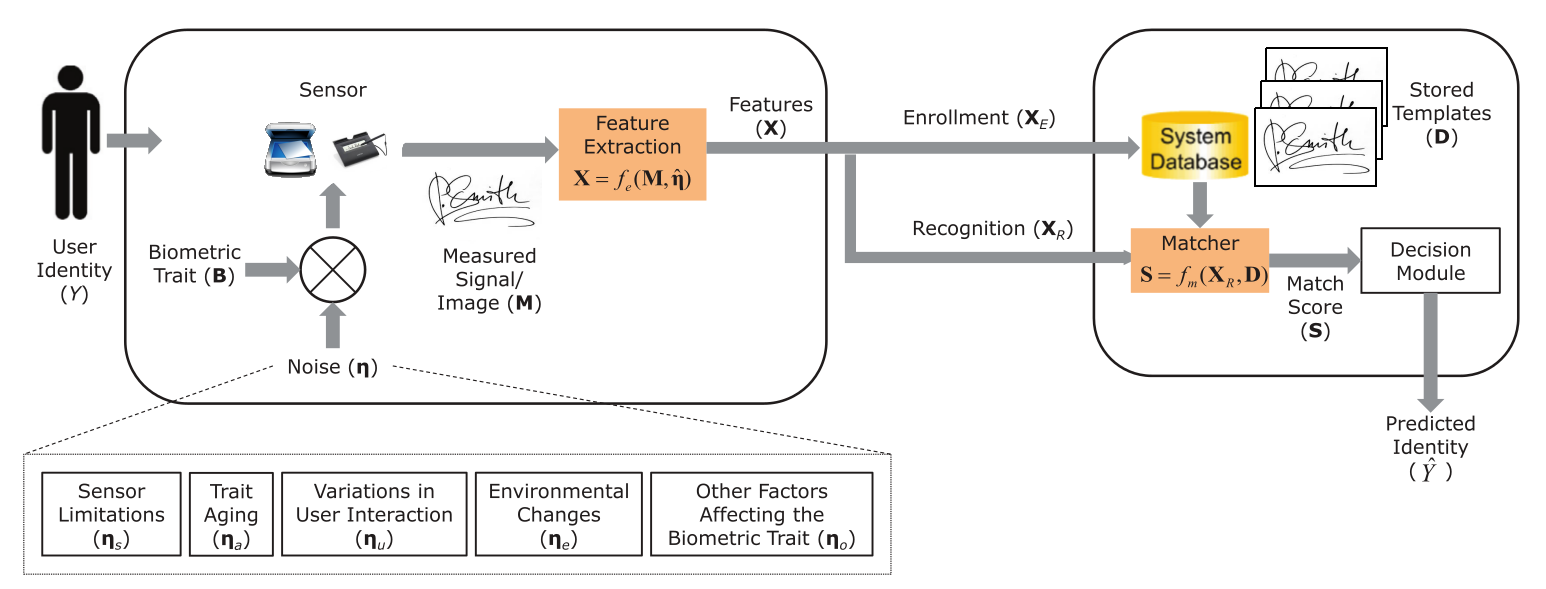
\includegraphics[width=\textwidth]{biometry-overview}
\caption{Overview of a typical handwritten signature based system. Figure adapted from \cite{jain2016}.}
\label{fig_ahsv-overview}
\end{figure}

As Figure \ref{fig_ahsv-overview} shows, the signature acquisition sensor can be either an optical scanner or an acquisition device such as a digitizing tablet. These two different acquisition tools characterize the two classes of signatures, namely: static and dynamic. 

In the static modality, also referred to as offline, an optical scanner is used to obtain the signature directly from the pen on the paper, and only the digital image of the signature is available, see Figure \ref{fig:acquisition} (a). In the dynamic mode, also called online, signatures are acquired through a graphic tablet or a pen-sensitive computer display, see Figure \ref{fig:acquisition} (b). In this mode, data is stored during the writing process and consists of a temporal sequence of the two-dimensional coordinates $(x, y)$ of consecutive points. 

\begin{figure}[!htpb]
\centering
 \subfloat[]{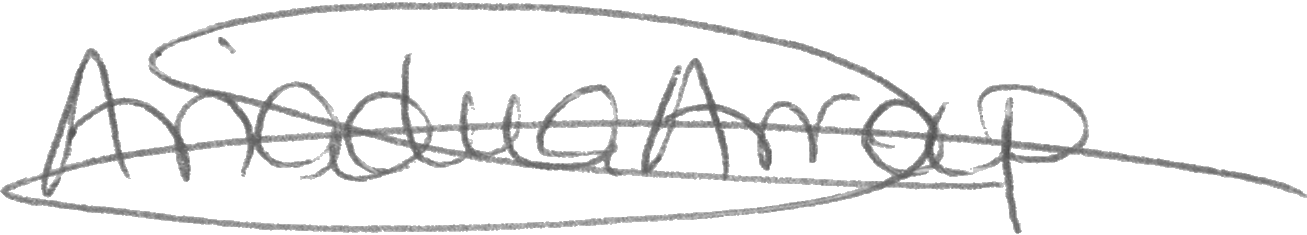
\includegraphics[width=3.2in]{signature.PNG}} 
\hspace*{0.5in} % separation between the subfigures
\subfloat[] {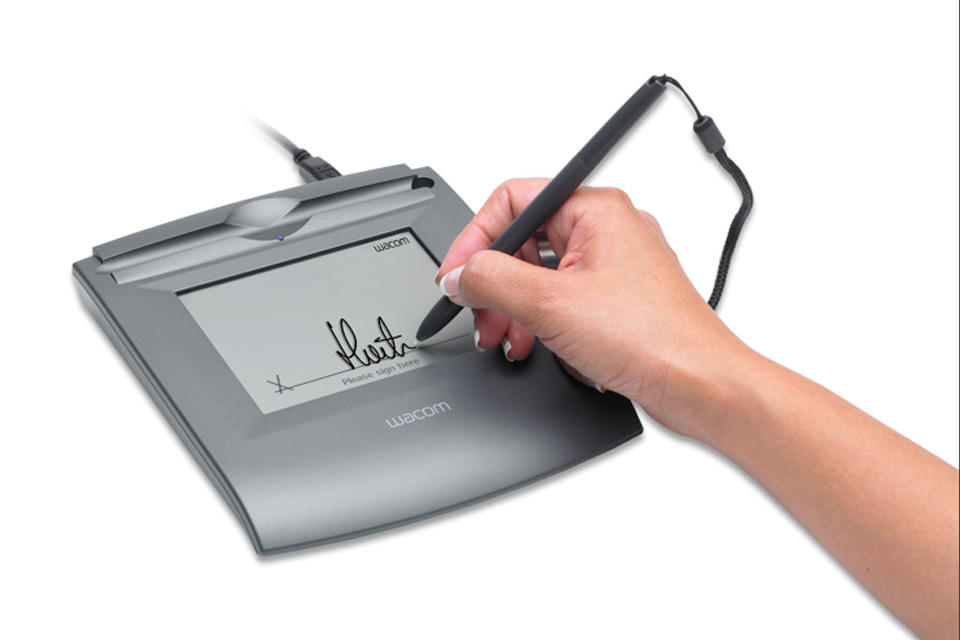
\includegraphics[width=2.7in]{stu500.jpg}}
\caption{Different signature acquisition methods. (a) a signature scanned from paper and (b) digitizing tablet Wacom STU-500 \cite{wacom2016}. } \label{fig:acquisition}
\end{figure}

Specifically, the online modality does not convey information about the overall shape of the signature, the width of the strokes and the texture of the ink on the paper \cite{diaz2014generation}. The offline representation, however, has lost all dynamic information about the manner in which the signature is signed during the acquisition process. As a result, features such as pen trajectory, which can be easily computed in the online domain, can only be inferred from a static image \cite{nel2005estimating}. An example of a colored offline signature and a plotted matching online signature can be found in Figure \ref{fig:offon}. 


\begin{figure}[!htb]
\centering
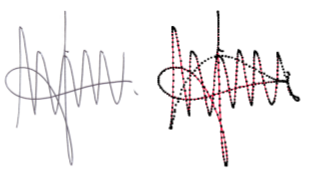
\includegraphics[width=3.8in]{offon}
\caption{An offline and a matching online signature sample. Figure extracted from \cite{sigcomp2009}.}
\label{fig:offon}
\end{figure}

%O pré-processamento tem como objetivos principais a correção de distorções
%geométricas na imagem e a remoção de ruídos, bem como a segmentação que é o
%processo de divisão da assinatura em múltiplas partes. É usualmente utilizada para
%identificar objetos ou outras informações relevantes em representações digitais.
%
%Na fase de classificação, os dados obtidos na extração devem ser utilizados para
%distinguir de forma inteligente entre assinaturas verdadeiras e falsas. Para este fim,
%existem diversas técnicas consagradas, como exemplo podemos citar as Redes Neurais
%Artificiais, HMM, SVM, DTW, entre outros. Além disso, modelos híbridos (junção de
%duas ou mais técnicas) poderão ser investigados para este objetivo.

Once the signature sample is acquired, during the enrollment phase, the system tries to create the subject identity based on behavioral features in the signature. Because of the way we sign, however, it is a subtle task. The rapid movement behind the signature creation is determined by a motor program stored in the brain of each signer applied to tools such as the pen on the paper \cite{pirlo2014advances}. According to \cite{plamondon1989automatic} there is a wide variety of human and social aspects that might affect the way we produce our handwritten signature, it might be influenced by country, age, time, habits, psychological or emotional state. The variability created on the signing process must be taken into account in the signature authentication process.

In fact, the unpredictable intra-personal variability, i.e. the similarity between signatures executed by the same writer, is a crucial challenge of signature-based biometric systems. This variability can be attributed to the several sources of noise ($\eta$) that distort the measured trait. According to Figure \ref{fig_ahsv-overview}, the intra-personal variability affecting the measured sample {\boldm $M$} can be characterized by several variables. These variables include sensor limitations such as resolution or sample rate; biological aging effects or cognitive-motor impairments; user interaction with the sensor; environment changes like background noise and other factors as consequence of the individuals’ mood, hurry or unwillingness to cooperate. The intra-personal variability effect is illustrated in Figure \ref{fig:intraclass}.

\begin{figure}[!h]
\centering
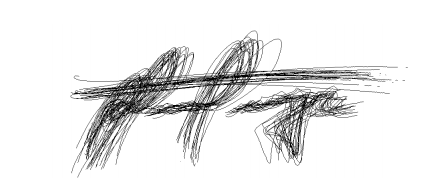
\includegraphics[width=5.2in]{superimposed}
\caption{Superimposed genuine signatures of the same writer. A high intra-personal variability can be noticed. Extracted from \cite{hafemann2015offline}. }
\label{fig:intraclass}
\end{figure}


Another challenge faced by signature-based biometric systems is the unpredictable inter-personal variability, i.e. the similarity between signatures executed by different writers. In a signature-based system, inter-personal variability is mainly attributed to frauds related to malicious people faking the identity of signers. Figure \ref{fig_forgeries} illustrates a visual comparison between genuine signatures and forgeries. 

\begin{figure}[!htb]
\centering
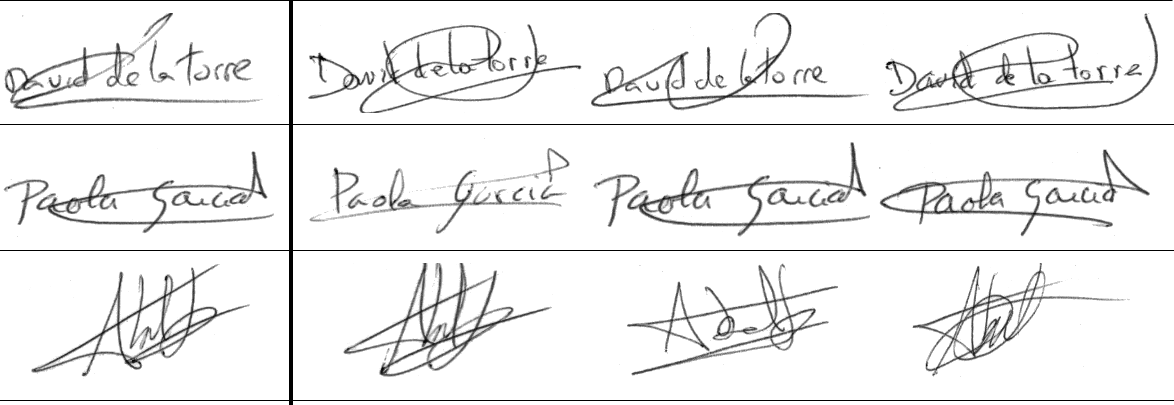
\includegraphics[width=\textwidth]{forgeries}
\caption[The first column of signatures are genuine references, the following three samples are questioned signatures. How many forgeries would you be able to detect? Signature images extracted from \cite{mcyt-100}.]{The first column of signatures are genuine references, the following three samples are questioned signatures. How many forgeries would you be able to detect?\protect\footnotemark Signature images extracted from \cite{mcyt-100}.} 
\label{fig_forgeries}

\end{figure}
\footnotetext{From left to right, top to bottom (F means Forgery and G means Genuine): FGF FFG GFF}

In the field of signature verification, forgeries are generally classified into two types. 
\begin{itemize}
\item The first one is the random forgery which is created in a situation which an impostor who has no information about the person or the shape of the original signature tries to verify the identity of a signer by using his genuine signature. The random forgery test is a typical test used in access control and commercial transactions. 

\item The second type is the skilled forgery, represented by a proper imitation of the genuine signature model. The forger has access for both the user’s name and signature, and learns the signature of a signer and tries to reproduce it with a similar intra-class variability. This test is the most relevant in signature verification for its impact in forensic applications in signature forgery detection. 
 
\end{itemize}




\section{Automatic Handwritten Signature Verification}
An Automatic Handwritten Signature Verification System (AHSVS) is conceptually a pattern recognition application. Pattern recognition is one of the most important and active fields of research. During the past few decades, there has been a considerable growth of interest in problems of pattern recognition, and in the last few years, many methods have been developed in this area, in particular on handwriting recognition and signature verification \cite{book}. 

As any Pattern Recognition system, an AHSVS has three phases: data acquisition and pre-processing, feature extraction and classification \cite{impedovo2008state}.

In the first step, the signatures are acquired and preprocessed, the main goal here is to convert them into a format suitable for the modeling process, correcting geometric distortions and removing noise related to the signature acquisition sensor. Afterwards features are extracted and stored in a knowledge database.  On the classification step, the extracted features are used to distinguish between genuine and forged signatures. Therefore the Signature Verification task is, in essence, a two-class classification problem, in which the system's prediction to the input signature sample is either genuine or fraud.

Verification errors occurring in AHSVS are usually categorized as two types \cite{fairhurst1997signature}. On the one hand, a genuine signer may be rejected by the system as a potential impostor (e.g. it could happen when the signer carelessly executes his/her signature), resulting in what is denoted a Type-1 error or False
Rejection. On the other hand, a skilled forger might be able to produce a sample which would be accepted as genuine, resulting in what is called a Type-2 error or False Acceptance. 

In order to improve the performance of signature verification
systems, bigger databases are required. The amount of data available for each user is often
insufficient in real applications. During the enrollment phase,
users are often required to supply only a few samples of their
signatures. In other words, even if there is a significant number
of users enrolled in the system, a classifier needs to perform
well for a new user, for whom only a small set of samples are
available. Since the acquisition
and distribution of real signatures arise legal and privacy
concerns, the use of realistic synthetic signatures could be
regarded as a good alternative. 

\section{Off-line Signature Synthesis Using On-line Samples}
One could synthesize an offline signature 2D image by interpolating the tracing, using a spline function for instance, between the digitized online points in addition to some morphological operators to enlarge the tracing to the desired stroke width. However, grayscale information would still be missing. 

TODO - quero colocar aqui uma visão geral das propostas existentes do estado da arte

assessment \cite{guest2013assessment}

rabasse 2008 \cite{rabasse2008new}

ferrer synthetic online to synthetic offline \cite{ferrer2013realistic}

\cite{diaz2014generation}

\cite{diaz2014cognitive}

%There are proposals in the literature focused on the generation of signature
%images from online signatures (Ferrer et al., 2013b; Guest et al., 2014; Rabasse et al.,
%2008). The common tendency is to apply different methods to dynamic signatures since
%these record the kinematic and the timing order in which the traces were registered.
%Once a new trajectory is obtained, the samples of the new specimen are interpolated in
%order to create new images. Then, an offline automatic classifier is used to assess the
%performance improvement. Parallel to this approach, a method of generating enhanced
%synthetic signatures images has been formulated using a novel architecture to improve
%the performance of dynamic verifiers (Galbally et al., 2015).
 %!TEX root = ../dissertation_vkslm.tex

\chapter{Neural Networks and Deep Learning} \label{ch:nndl}
This chapter introduces and gives a brief overview of the theoretical foundations of Deep Neural Networks. In the first section, basic concepts of Artificial Neural Networks are presented, starting from the original models. The next section gives an introduction and a general overview of the deep learning research field, discussing the recent advancements that enabled training Deep Neural Networks successfully. Finally, we briefly describe the fundamentals of the Convolutional Neural Network and present the Fully Convolutional Networks, which is a model used in this work, and we present the techniques used for training our model.

\section{Artificial Neural Networks}

A biological neural network is an essential part of human brain. The human brain is a highly complex information processing system capable of interpreting large amounts of information and making decisions. It is a complex, non-linear and parallel ``computer'' consisting of millions of connected neurons \cite{haykin2009neural}. In many tasks, the human brain is more efficient than computers. For instance, the human brain can recognize a familiar face in about 100-200 ms, while modern computers require minutes or even hours for solving the same problem \cite{haykin2009neural}.

Based on examples and feedback from the ``teacher'', our brain allows us learning how to
distinguish an apple from an orange or recognize letters. Moreover, even without the ``teacher'', we are still able to group similar patterns. Those and other strengths of human brain challenged scientists to emulate those processes by researching how to use machines for tasks that are common for humans. Moreover, one of the concepts that appeared as the result of that research is the Artificial neural network (ANN) concept. 

\subsection{Artificial Neuron}
The first model to simulate a single neuron, which is the elemental building block of neural networks, was the perceptron \cite{rosenblatt1958perceptron}. A single neuron implements a mathematical function given its inputs, to provide an output, as described in Equation \ref{eq:activation} and illustrated in Figure \ref{perceptron}.
\begin{equation}
y = f(\sum_{i=1}^{n} x_{i}w_{i} + b)
\label{eq:activation}
\end{equation}

In this equation, $x_{i}$ is the input $i$, $w_{i}$ is the weight associated with input $i$, $b$ is a
bias term and $f$ the activation function. 
\begin{figure}[!htb]
\centering
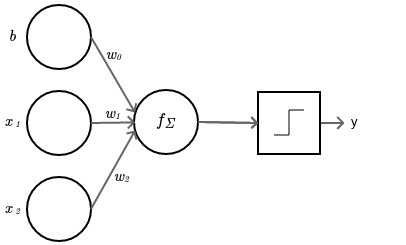
\includegraphics[width=3.4in]{perceptron}
\caption{Perceptron representation. $x_{1}$ and $x_{2}$ represent the input signal, $b$ the bias term, $w_{0}$, $w_{1}$, $w_{2}$ the weights, $f_{\:\sum}$ is the activation function (in this case, a step function) and the output signal is given by $y$.}
\label{perceptron}
\end{figure}

%The learning rule algorithm for learning relations in data with a neuron can be summarized as: for every input $x_{i}$, make a linear prediction about its label: $y^*_{i} = w^T x_{i}$
%and update the weights ($w$) as,
%\begin{equation}
%w \leftarrow w + x_{i}(y_{i} - y^*_{i})
%\end{equation}


Models based on perceptrons have severe limitations. An evaluation by Minsky and Papert \cite{papert1969perceptrons} showed that a perceptron cannot model data that is not linearly separable, such as a simple XOR operator. It was observed that ``for data sets that are not linearly separable, the perceptron learning algorithm will never converge'' \cite{bishop2006pattern}. This observation is related to the perceptron's limited representational power, the learning rule only converges to the correct solution if the data is linearly separable. The Multilayer Perceptron (MLP) with a single hidden layer, however, has been proven \cite{hornik1989multilayer} to approximate any continuous function on a compact input domain to arbitrary precision. For this reason, MLPs are said to be \textit{universal function approximators} \cite{hornik1989multilayer}.

\section{Multi-layer Neural Networks}
Multi-layer Neural Networks such as the MLP consist of stacking several neuron units together. Specifically, in the MLP, neurons are stacked in one layer connecting these stacks sequentially, without connections between the neurons in the same layer, as it is shown in Figure \ref{mlp}. Each neuron in the MLP is normally fully connected with all the neurons in the next layer, with its own set of weights. The first layer of an MLP is usually the input sample, and the last layer is the output of the network. The layers between the input and output layers are called hidden layers.

\begin{figure}[!htb]
\centering
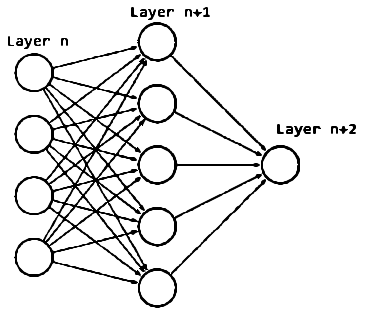
\includegraphics[width=0.5\textwidth]{mlp}
\caption{Multilayer perceptron representation. Each layer contains several perceptron units, which are then connected to units in the subsequent layer.}
\label{mlp}
\end{figure}

An MLP can be thought of as a function that maps from input to output vectors, parameterized by the neuron connection weights. The output of a layer
is calculated by applying the neuron activation function for all neurons on the layer, as
noted in Equation \ref{eq:outputmlp}
\begin{equation}
y^{(l)} = f(W^{(l)} y^{(l-1)} + b^{(l)})
\label{eq:outputmlp}
\end{equation}
where $W^{(l)}$ is a matrix of weights assigned to each pair of neurons from layer $l$ and $l-1$, and $b^{(l)}$ is a vector of bias terms for each neuron in layer $l$. Calculating the output starting from the first hidden layer, up to the output layer is also referred to as the \textit{forward propagation} phase.

\subsection{Loss Function}
%control c control v
In order to train the model, an objective function, also called loss function, is defined.
This function measures the compatibility between a prediction (e.g., the class scores in classification) and the ground truth label. The
objective of the training is to minimize the sum (or, equivalently, the mean) of
this error function applied to all examples in the dataset. Commonly used loss functions
are the Mean Squared Error function (MSE), and the Cross-Entropy (CE). Equations \ref{eq:mse} and \ref{eq:ce} describe the MSE and CE, respectively, for a sample of the dataset,

\begin{equation}
E =  \frac{1}{N} \sum_{c}^{N} (t_{(c)} - y^{}_{(c)} )^2 
\label{eq:mse}
\end{equation}

\begin{equation}
E = - \sum_{c}^{N} (t_{(c)} \: log \: y^{}_{(c)} )^2 
\label{eq:ce}
\end{equation} where $y^{}_{(c)}$ is the output of unit $c$ in the last layer, $t_{(c)}$
the true label $t$ for unit $c$ and $N$ is the number of units on the last layer.
\subsection{Backpropagation}
The phase called backpropagation consists in minimizing the error $E$ between the network output and the expected target. The algorithm works by calculating the derivatives of the error
function with respect to the model’s parameters (weights and biases). Then, it propagates the error from the output layers, back to the initial layers, one layer at a time, in order to update the weights of the neuron connections to minimize the error $E$. The weights are updated conforming Equation \ref{eq:bp}

\begin{equation}
w(t+1) = w(t) - \alpha\ \Delta\ E(w(t))
\label{eq:bp}
\end{equation}
where $E$ is the error measure defined as loss sum over the entire training set, and $t$ indicates iterations (time steps). The $\Delta(E)$ is the gradient vector, which is computed by applying the chain rule on the layers of the NN \cite{rumelhart1985learning}. The parameter $\alpha$ is a heuristic, called learning rate. The learning rate values help to avoid convergence to a local-minimum or maximum point. In order to secure the convergence of the backpropagation training algorithm and avoid oscillations in a steep direction of the error surface, a small learning rate is chosen $(0 < \alpha < 1)$.

\subsection{Activation Functions}
\begin{figure}[!htb]
\centering
 \subfloat[Sigmoid]{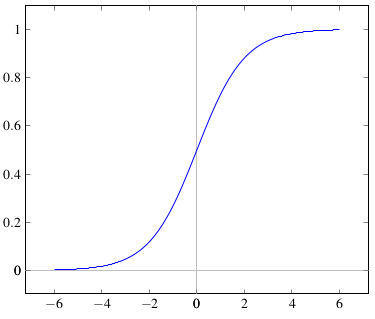
\includegraphics[width=2.5in]{sigmoid}} 
\hspace*{0.2in} % separation between the subfigures
\subfloat[Tanh] {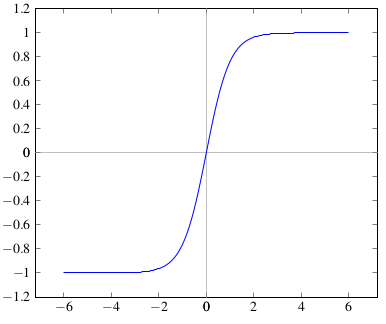
\includegraphics[width=2.5in]{tanh}}
\\
\subfloat[ReLU] {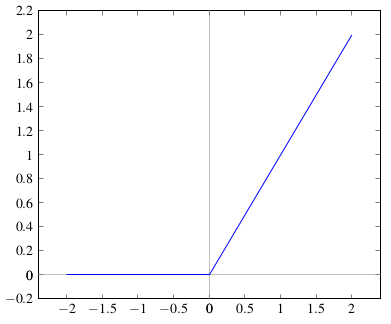
\includegraphics[width=2.5in]{relu}}
\hspace*{0.2in} % separation between the subfigures
\subfloat[LReLU] {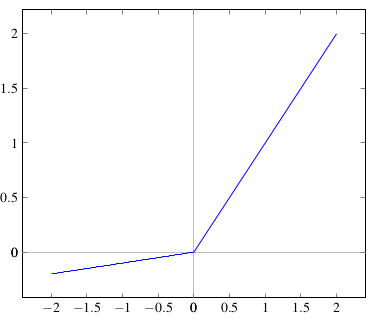
\includegraphics[width=2.5in]{lrelu}}


\caption{Neural network activation functions. } \label{fig:activation}
\end{figure}
\subsubsection{Sigmoid}
The sigmoid activation function is a non-linear function in the range of $]0, 1[$ and has the mathematical form defined in Equation \ref{eq:sigmoid} and is shown in the Figure \ref{fig:activation} (a).
\begin{equation}
f(x) = \frac{1}{1+e^{-x}}
\label{eq:sigmoid}
\end{equation}
It takes a real-valued number and transforms it to the range between 0 and 1. Small negative numbers become 0 and large positive numbers become 1. 
\subsubsection{Tanh}

The Hyperbolic Tangent (tanh) non-linearity is shown in Figure \ref{fig:activation} (b) and is defined in Equation \ref{eq:tanh}. It limits a real-valued number to the range of $[-1, 1]$
\begin{equation}
f(x) = \frac{e^x - e^{-x}}{e^x + e^{-x}}
\label{eq:tanh}
\end{equation}

\subsubsection{Rectified Linear Unit}

The Rectified Linear Unit (ReLU) has become very popular in the last few years and was one of the main discoveries that enabled the training of deeper neural networks. It computes the function 
\begin{equation}
f(x)=max \: (0,x)
\label{eq:relu}
\end{equation}
in other words, the activation is simply thresholded at zero, see Figure \ref{fig:activation} (c). 

\subsubsection{Leaky Rectified Linear Units}

Leaky Rectified Linear Units (LReLU) is an attempt to improve the ReLU. Instead of the function being zero when $x < 0$, a leaky ReLU will instead have a small negative slope (around 0.01). The function computes

\begin{equation}
f(x)=\begin{cases}
      \alpha x, & \text{if}\ x < 0\\
      x, & \text{otherwise}
    \end{cases}
\label{eq:lrelu}
\end{equation} where $\alpha$ is a small constant, see Figure \ref{fig:activation} (d). 


\section{Deep Neural Networks}
Deep architectures are characterized by the multiple levels of non-linear operations
contained on a neural network. While many of the early successful applications of neural networks used shallow architectures (up to 3 hidden layers). It was found, however, that the mammal brain is organized in a deep architecture. The brain appears to process information through multiple stages, which is particularly clear in the primate visual system \cite{bengio2009learning}. 

It was observed in many experiments that deep networks are harder to train than shallow networks, and that training deep networks often get stuck in apparent local minima (or plateaus) when starting with random initialization of the network parameters. Deep Neural Networks have been investigated for decades, but training deep networks consistently yielded poor results. 

The proposal of the Convolutional Neural Network \cite{lecun1995convolutional} and some recent theoretical discoveries made training deep neural networks feasible. The CNN is a particular type of deep, feedforward neural network that is easier to train and generalized better than networks with full connectivity between adjacent layers \cite{lecun2015deep}. Besides, the theoretical findings include unsupervised training of the layers \cite{hinton2006fast}, Rectifier Linear Unit (ReLU) \cite{nair2010rectified} as the activation function and the regularization techniques Dropout \cite{srivastava2014dropout} and Batch Normalization \cite{ioffe2015batch}. 


\section{Convolutional Neural Networks}
CNNs combine three architectural ideas: local receptive fields, shared
(tied) weights and spatial or temporal sub-sampling \cite{lecun1998gradient}. When trained with appropriate regularization, CNN achieves state-of-the-art performance
on visual object recognition and image classification tasks \cite{lecun2015deep}. The CNN is composed of several layers of trainable filters (convolutional layers) and local neighborhood pooling operations (pooling layers) stacked in an alternating sequence starting with the raw input images. To illustrate the concept, Figure \ref{lenet} shows an example of an architecture of a CNN, namely, the Lenet \cite{lecun1998gradient}, one of the first applications of the CNN used for handwriting recognition.

\begin{figure}[!htb]
\centering
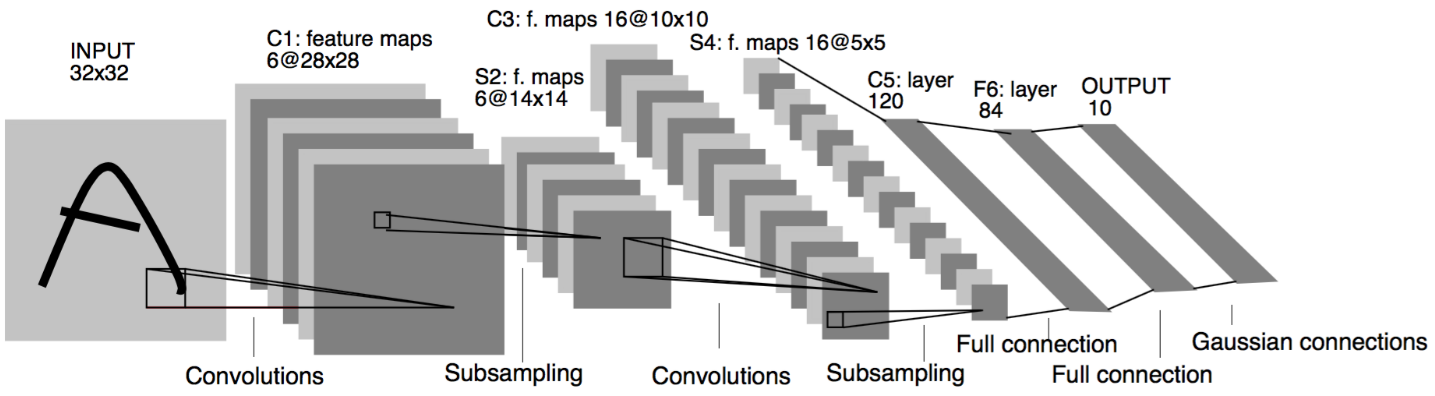
\includegraphics[width=\textwidth]{lenet}
\caption{Lenet \cite{lecun1998gradient}, a convolutional neural network used for handwriting recognition.}
\label{lenet}
\end{figure}

Figure \ref{learned} provides an example of the filters learned on a convolutional layer of a network trained for object classification, showing that this type of architecture is
capable of learning interesting feature detectors, similar to edge detectors.
\begin{figure}[!htb]
\centering
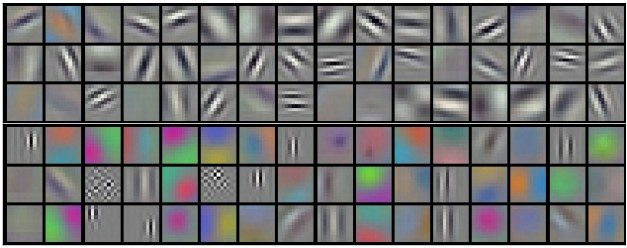
\includegraphics[width=0.7\textwidth]{learned}
\caption{Example of feature maps learned by the CNN proposed by \cite{krizhevsky2012imagenet} for object classification.}
\label{learned}
\end{figure}


\subsection{Convolutional Layer}
Convolutional layers have trainable filters (also called feature maps) that are applied
across the entire input \cite{lecun1995convolutional}. For each filter, each neuron is connected only to a subset of
the neurons in the previous layer. In the case of 2D input (such as images), the filters
define a small area (e.g., 3x3 or 5x5 pixels), and each neuron is connected only to the
nearby neurons (in this area) in the previous layer. The weights are shared across neurons,
leading the filters to learn frequent patterns that occur in any part of the image.

The definition for a 2D convolution layer is presented in Equation \ref{eq:cnn}. A 2D convolution layer is the application of a discrete convolution of the inputs $y^{(l-1)}$ with a filter $w^{(l)}$, adding a bias $b_{(l)}$ , followed by the application of an activation function $f$:

\begin{equation}
y^{(l)}_{rc} = f(\sum_{i=1}^{N_{r}} \sum_{j=1}^{N_{c}} y^{(l-1)}_{(r+i-1)(c+j-1)} w^{(l)}_{ij} + b^{(l)} )
\label{eq:cnn}
\end{equation}
where $y^{(l)}_{rc}$ is the output at position $\{r,c\}$, $N_{r}$ and $N_{c}$ are the number of rows and columns, respectively, of the 2D filter, $w^{(l)}_{ij}$ is the filter value at position $\{i,j\}$, $y^{(l-1)}_{(r+i-1)(c+j-1)}$ is the $\{r+i-1,c+j-1\}$.


The equation above is defined for all possible applications of the filter, as in Figure \ref{fig:convop} (a), that is, for
$r \in \{1, ..., I_{r} - N_{r} + 1\}$ and $c \in \{1, ..., I_{c} - N_{c} + 1\}$, where $I_{r}$ and $I_{c}$ are the number of rows and columns in the input to this layer. The convolutional layer can either apply the filters for all possible inputs \footnote{Animated representation can be found in: \url{https://raw.githubusercontent.com/vdumoulin/conv_arithmetic/master/gif/no_padding_no_strides.gif}}, or use a different strategy. Instead of applying the filter for all possible $\{r, c\}$ pairs, only the pairs with distance
$s$ are used, which is called the stride. A stride $s = 2$ \footnote{Animated representation of strides can be found in: \url{https://raw.githubusercontent.com/vdumoulin/conv_arithmetic/master/gif/no_padding_strides.gif}} is equivalent to apply the convolution for half of the possible pairs, as in Figure \ref{fig:convop} (b).

\begin{figure}[!htb]
\centering
\subfloat[Convolving a 3x3 kernel over a 4x4 input, with 1x1 stride.] {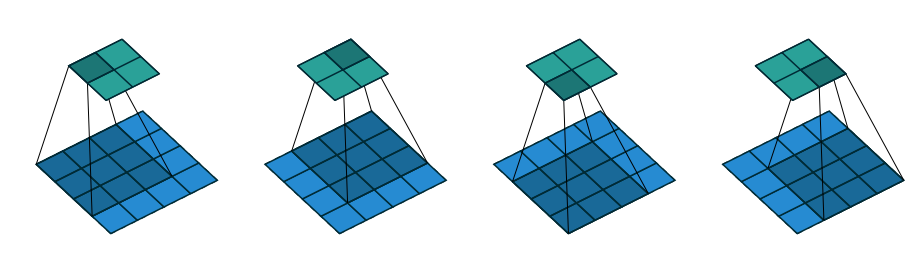
\includegraphics[width=\textwidth]{conv-operation}}
\\
\subfloat[Convolving a 3x3 kernel over a 5x5 input, with 2x2 stride.] {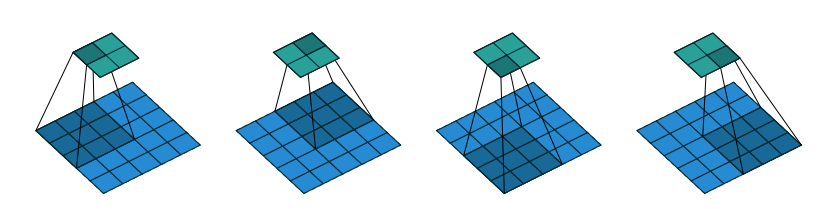
\includegraphics[width=\textwidth]{conv-operation-strides}}


\caption{Convolution operation with (a) stride 1x1 and (b) stride 2x2. Extracted from \cite{dumoulin2016guide}.} \label{fig:convop}
\end{figure}


\section{Fully Convolutional Network Architecture}

The Fully Convolutional Network (FCN) \cite{long2015fully} is a CNN modified for dense
predictions. This architecture was developed under the observation that although a typical CNN is designed for spatial inputs, such as images, it normally discard spatial information in their fully connected layers (FC). 

FCNs are, thus, rooted in the observation that spatial filters, which are learned during the CNN training, are useful for extracting low-level features, but FC layers are needed to incorporate high-level reasoning. The main idea of the FCN architecture is to convert the FC layers of a CNN into convolutional layers, expecting that the network retains the ability to learn high-level information and at the same time preserve spatial information. The FCN becomes, therefore, ``fully convolutional'' by having end-to-end convolutional layers. 

While CNNs are typically built in a sequence of convolutional, pooling, and fully connected layers, FCN adds an expanding path built with a transposed convolutional layer \cite{long2015fully}. The expanding path recovers spatial information by merging features skipped from the various resolution levels on the contracting path.

Unlike a CNN, which learns a general, nonlinear function that characterizes the input, FCNs learn an end-to-end nonlinear mapping from one input image to another. Because pixel-wise prediction is used, the label space is also transformed from a scalar to a two-dimensional image, where each pixel value represents the object class of its corresponding input pixel. An FCN with an input image and label is illustrated in Figure \ref{fcn-arch}


\begin{figure}[!htb]
\centering
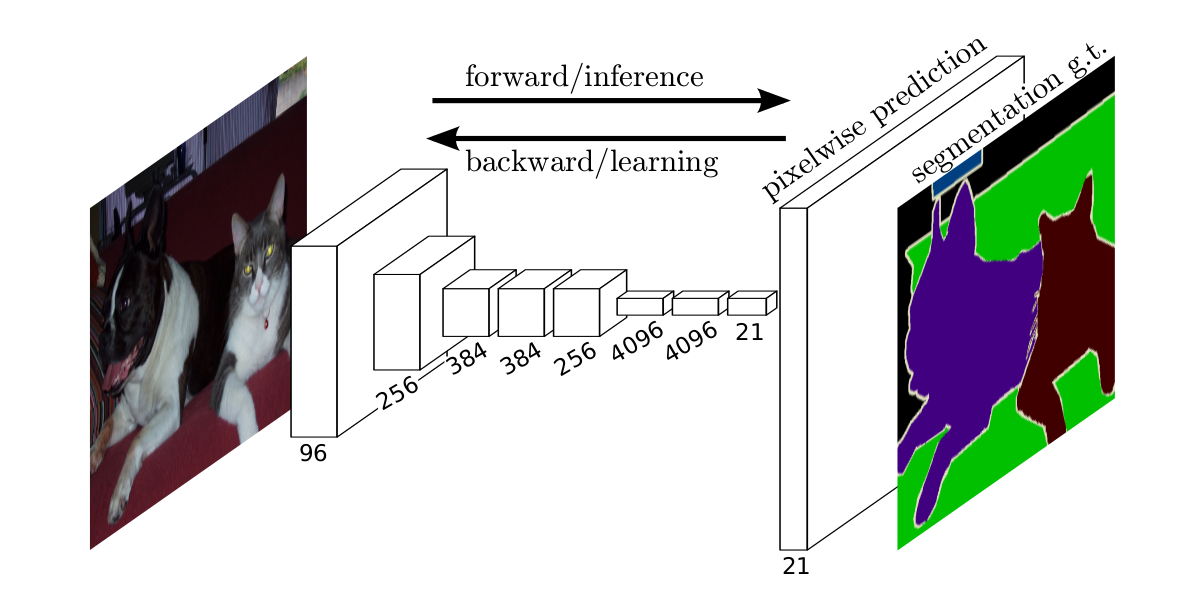
\includegraphics[width=\textwidth]{fcn-arch}
\caption{Fully convolutional networks can efficiently learn to make dense predictions for
per-pixel tasks. Extracted from \cite{long2015fully}}
\label{fcn-arch}
\end{figure}

\subsection{Transposed Convolution}
%https://arxiv.org/pdf/1603.07285.pdf p 19

Transposed convolutions - also called deconvolution or backward convolution - work by swapping the forward and backward passes of a convolution. One way to put it is to note that the kernel defines a convolution, but whether it is a direct convolution or a transposed convolution is determined by how the forward and backward passes are computed \cite{dumoulin2016guide}.

For instance, one might use such a transformation as the decoding layer of an FCN or project feature maps to a higher-dimensional space. Figure \ref{fig:transposed} illustrates the general backwards convolution process \cite{dumoulin2016guide}.

\begin{figure}[!htb]
\centering
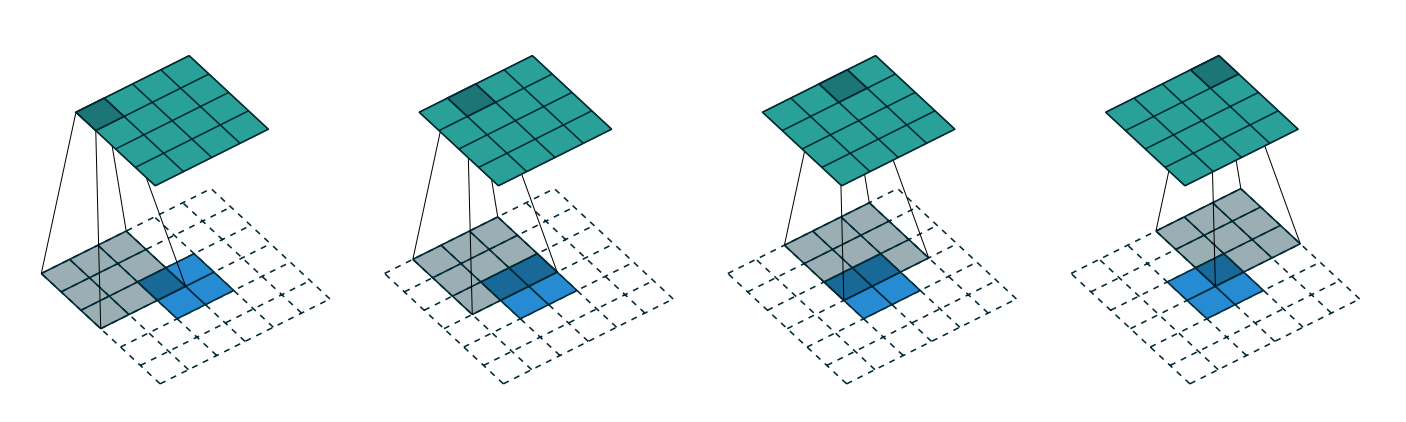
\includegraphics[width=\textwidth]{transposed}

\caption{Upsampling with transposed convolutions. Upsampling is done by padding
(white) the original pixels (blue) and convolving them with a filter (gray). The result is
an upsampled image (green). Here a stride of one is used, illustrated from left to right. Extracted from \cite{dumoulin2016guide}.} \label{fig:transposed}
\end{figure}

\section{Deep Neural Networks Training}

\subsection{Weight Initialization}
When the training of the neural network starts, the initial values of the weights and biases need to be provided. Some techniques to weight initialization have been proposed and shown to be useful to smooth the model convergence.

\subsubsection{Uniform}
The uniform initialization is the most simple. The model parameters are initialized through a random distribution in the range of $[l1, l2]$, where $l1$ and $l2$ are two constants.

\subsubsection{Glorot}
This weight initialization technique was proposed in \cite{glorot2010understanding}. The dynamic of the activation functions and the gradients weights were studied, and they found the neural network converges faster using the weight initialization described in Equation \ref{eq:glorot}.

\begin{equation}
W \sim U \; \left[\sqrt{\frac{6}{f_{in}+f_{out}}}\; \right] 
\label{eq:glorot}
\end{equation}
where $W$ are the weights, $U$ is an uniform distribution, and $f_{in}$ and $f_{out}$ are the number of units in the previous layer and the next layer, respectively.

\subsection{Optimization Algorithms}
Training the network consists in minimizing the error function, based on the gradients of the parameters with relation to the cost function, by updating the weights and biases, expecting that the network learns how to perform the task it is being trained for.

\subsubsection{Stochastic Gradient Descent}

The Stochastic Gradient Descent (SGD) algorithm, as defined in \cite{bishop2006pattern} can be summarized a series of iterations over mini-batches of the dataset, performing forward-propagation
followed by a back-propagation to calculate the error derivatives with respect to the parameters. The weights are updated using these derivatives, and a new mini-batch is used. This procedure is repeated until a convergence criterion is  reached. Common convergence criteria are a maximum number of epochs (number of times that the whole training set was used); a desired value for the cost function is reached, or training until the cost function shows no improvement in a number of iterations.

\subsubsection{Adaptive Moment Estimation}
The Adaptive Moment Estimation (ADAM) \cite{kingma2014adam} is a stochastic optimization method that can adaptively tune the learning rate per parameter and also keeps an exponentially decaying average of past gradients $m_t$ and $v_t$:

\begin{subequations}
\begin{gather}
\label{adamfirst}
m_t = \beta_1 m_{t-1} + (1 - \beta_1) g_t \\   
v_t = \beta_2 v_{t-1} + (1 - \beta_2) g_t^2  
\end{gather}
\end{subequations}
where $m_t$ and $v_t$ are estimates of the first moment and the second moment of the gradients respectively, $\beta_1$ and $\beta_2$ are the decay rate and $g$ is the gradient with respect to $w$. 

The authors observed that the moments are biased towards zero, especially during the initial time steps. They work around these biases by computing bias-corrected estimates:
\begin{subequations}
\begin{gather}
\hat{m}_t=\dfrac{m_t}{1 - \beta^t_1} \\
\hat{v}_t=\dfrac{v_t}{1 - \beta^t_2}
\label{adamend}
\end{gather}
\end{subequations}
Then, they use these computed variables to update the parameters:
\begin{equation}
w_{t+1} = w_{t} - \alpha \dfrac{\hat{m}_t}{\sqrt{\hat{v}_t} + \epsilon} 
\label{adamend2}
\end{equation}
The authors propose default values of 0.9 for $\beta_1$, 0.999 for $\beta_2$, and $10^{-8}$ for $\epsilon$.



%!TEX root = ../dissertation_vkslm.tex

\chapter{Proposed Method}\label{ch:method}


Given a dynamic signature, the simplest way to obtain the corresponding static sample is to draw $(x, y)$ coordinates and performing a simple interpolation in order to get a continuous trajectory. The problem of this approach is that other dynamic information (e.g. velocity, pressure, etc.) do not contribute in the transformation process, so that the offline version will result in a poor execution.

Some more complex methods have already been proposed, nevertheless, these methods are “rule-based”. Here we propose a method that learns from data how to perform the transformation having samples of both dynamic and static signatures. 

Figure \ref{fig_method}  shows the workflow of the proposed approach to generate a static signature-based on online data. In this chapter, we describe our proposed method. First, the dataset used to train our model is described, then we describe how we preprocessed the dataset. Afterwards, the FCN model trained to learn an end-to-end mapping from the dynamic information to the static representation of the signature is detailed.

\begin{figure}[!htb]
	\centering
	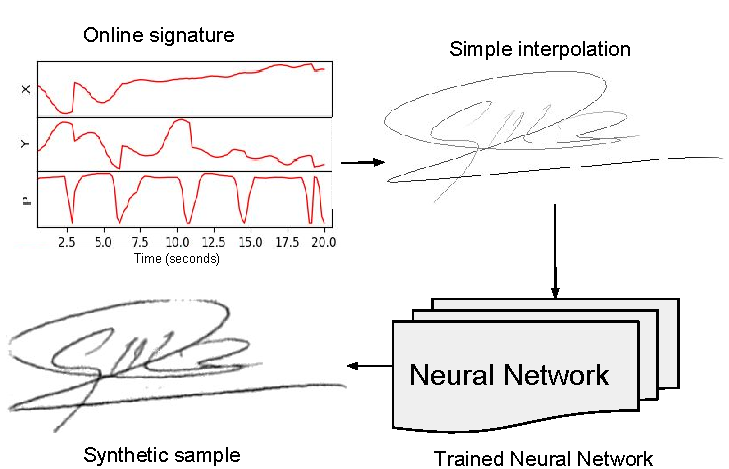
\includegraphics[width=4.6in]{method}
	% where an .eps filename suffix will be assumed under latex,
	% and a .pdf suffix will be assumed for pdflatex; or what has been declared
	% via \DeclareGraphicsExtensions.
	\caption{The proposed approach diagram and an example of the synthetic signature generation.}
	\label{fig_method}
\end{figure}



\section{Online to Offline Training Data}
In order to train our Neural Network to perform the approximation task of ``online to offline conversion,'' we need both the online version of a manuscript containing the trajectory and pressure information mapped to the respective resulting offline representation, as in Figure \ref{fig:offon}. Of course the mapping is a major problem since the two acquisition systems (digitizing tablet and optical scanner) process the writing signal separately, each having its particular parameters (Cartesian axis, scale, etc.). 

Moreover, the acquisition phase of such dual dataset requires some extra steps. A paper form must be placed over a digital tablet to be filled with an electronic ink-pen. Then, the dynamic data is captured through the tablet, and the paper form might be scanned to provide the offline image, Figure \ref{fig:dualonoff} illustrates this setup. Thereby, two complementary files are available. One contains the dynamic information, and the other one is the digital image of this piece of handwritten signature produced by the scanner. 
\begin{figure}[!htb]
\centering
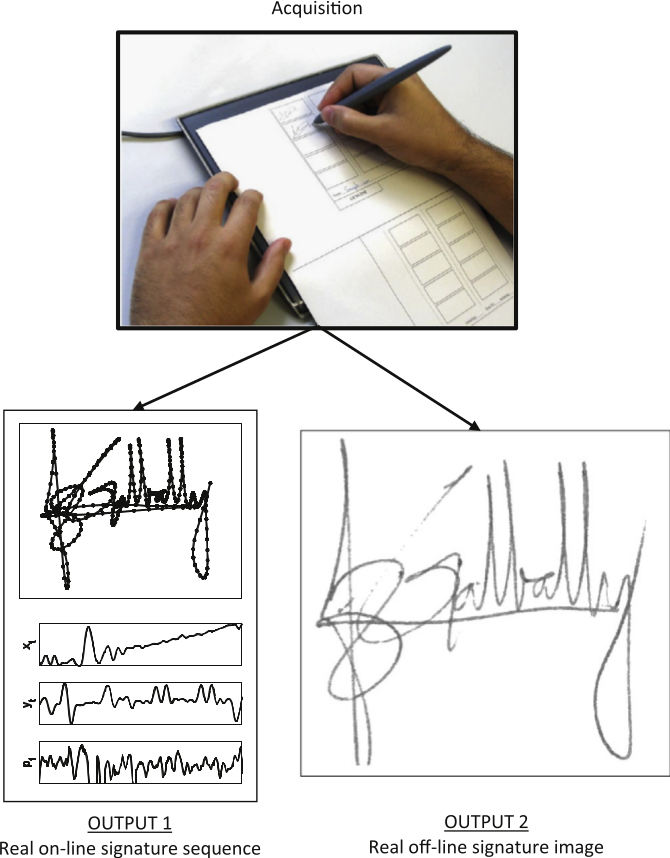
\includegraphics[width=0.7\textwidth]{dualonoff}

\caption{An user signing on a paper placed over a digitizing tablet. This way, the dynamic and static versions of the same signature are acquired simultaneously. Figure extracted from \cite{galbally2015line}}
\label{fig:dualonoff}
\end{figure}

In order to project the online signature in the respective offline version, these two types of information should be available within the same coordinate system, with the same origin, the same resolution, and orientation. However, as the two acquisition systems (tablet and scanner) are processing the writing separately and with their particular parameters, this assumption is not satisfied directly. Geometrical transformations have to be applied to compensate for these differences. To the best of our knowledge, however, the creators of the publicly available dual modal signature datasets \cite{biosecurid, biomet, myidea, sigcomp2009, sigma, sigwicomp2013, sigwicomp2015} had not this characteristic satisfied. As it can be seen in Figure \ref{fig:onoff}, both of the representations of the signatures do not match if we plot it in a single image.

\begin{figure}[!htb]
\centering

\includegraphics[width=0.5\textwidth]{onoff}
% where an .eps filename suffix will be assumed under latex, 
% and a .pdf suffix will be assumed for pdflatex; or what has been declared
% via \DeclareGraphicsExtensions.
\caption{A sample from the BiosecurID dataset. Here we can see that the online signature (interpolated in red) can not be projected in the respective offline version.}
\label{fig:onoff}
\end{figure}

The dual domain IRONOFF \cite{viard1999ireste} handwriting dataset was thus used to train our model. Besides acquiring both domains of the handwriting manuscript, the online data is mapped to the same coordinate system of the offline data, as shown in Figure \ref{fig:ironoff-mapped}, the interpolated online data is shown in white. Using this dataset, we make the fair assumption that a handwritten signature is a manuscript. With that in mind, we expect that even if the network was trained on handwriting manuscripts, it would work for online signatures to generate its static version.

The IRONOFF dataset contains a total of 23000 mapped online and offline samples of the manuscripts. The offline handwriting signals have been sampled with a spatial resolution of 300 dots per inch (DPI), with 8 bits per pixel (256 gray level).

\begin{figure}[!htb]
\centering

\includegraphics{ironoff-mapped}
% where an .eps filename suffix will be assumed under latex, 
% and a .pdf suffix will be assumed for pdflatex; or what has been declared
% via \DeclareGraphicsExtensions.
\caption{An offline manuscript mapped with the respective online trajectory. Image extracted from \cite{viard1999ireste}.}
\label{fig:ironoff-mapped}
\end{figure}


\section{Preprocessing}
%Copy and paste
During the training of our FCN model, two 2D matrices are needed, the input and output. The input is the online information of the manuscript, and the output is the expected offline representation.

In order to create a 2D representation of the dynamic information of the manuscript, we create a simple linear interpolated version of the time-series ($x_{t}, y_{t}, p_{t}$) using the Bresenham line algorithm \cite{bresenham} to obtain the 8-connected sequences. As a result, we get an image in which the trajectory of the signature is represented by one pixel, where the pixel intensity is the pressure information.

Since the neural network expect inputs and outputs of a fixed size and the manuscripts shape vary significantly in the IRONOFF (they range from samples of width x height size of 167x214 to larger samples of size 548x215 pixels), we convert it to a fixed size. We follow an approach similar to what was previously proposed in the literature, e.g., \cite{pourshahabi2009offline}. First, we normalize the images to the largest image size, by padding the images with white background. Then, we center the manuscript in a canvas of size 548x215 pixels (the largest sample size in the dataset), aligning the center of mass of the sample to the center of the image. Finally, we rescale the images, using a bilinear interpolation, to 383x150 pixels, i.e., 70\% of the canvas size, maintaining the aspect ratio of the original sample. This size was chosen to be large enough to keep details from the pen strokes in the manuscript.

Besides resizing the images to a standard size, we also performed the following pre-processing steps:
\begin{itemize}
\item Inverted the images: we inverted the images so that the white background corresponded to pixel intensity 0. 
\item Normalized the input: we normalized the input to the
neural network by dividing each pixel by the standard
deviation of all pixel intensities. We do not normalize the data to have mean 0 (another common pre-processing step) since we want the
background pixels to be zero-valued.
 
\end{itemize}

Figure \ref{fig_ironoff} shows what is the result of the preprocessed input and the groundtruth being fed to the neural network during the training phase.



\begin{figure}[!htpb]
\centering
 \subfloat[input]{
\includegraphics[width=2.0in]{input-ironoff}} 
\hspace*{0.5in} % separation between the subfigures
\subfloat[ground truth] {
\includegraphics[width=2.0in]{gt-ironoff}}
\caption{Preprocessed data used during the training phase. (a) is the interpolated online sample, used as input and (b) is the expected prediction from the neural network, the ground truth. } \label{fig_ironoff}
\end{figure}



\section{Neural Network Model}

Our model is based on the fully convolutional neural network architecture, adopted to learn an end-to-end nonlinear mapping from online representation to the static image. Our Neural Network model is fed with the interpolated online sample pressure information and we expect the respective offline sample on the output, i.e., the input is the pressure information and the desired output is the static manuscript.

We use a simplified architecture based on the one proposed in \cite{long2015fully}. The expectation is that by learning to transform between online information to offline manuscripts, the network will learn convolution filters that are relevant to synthesize offline signatures based on the online sample.

Our convolutions architecture is a simplified version of the FCN-VGG \cite{long2015fully, simonyan2014very} and the transposed convolutions were symmetric to the convolution operations. We used a simplified version because during some initial tests we observed that the capacity of the original network architecture seemed to be too large for the problem at hand, particularly considering the amount of convolutional operations. We observed that the model was not learning useful transformations on the first few epochs. We obtained better results with the simplified architecture presented in Table \ref{table:cnn-arch}. 

For the purpose of replicating our experiment, we provide the list of the parameters used in our tests. Table \ref{table:cnn-arch} lists the definition of the FCN layers. For convolution and transpose convolution layers, we list the size as NxHxW where N is the number of filters, H is the height and W are the width of the layer window.

\begin{table}[!htb]
\renewcommand{\arraystretch}{1.3}
\caption{Summary of the CNN Layers}
\centering
\begin{tabular}{|l|l|}
\hline
\textbf{Layer}        & \textbf{Size} \\ \hline
Convolution           & 16x3x3        \\ \hline
Convolution           & 32x3x3        \\ \hline
Convolution           & 32x3x3        \\ \hline
Convolution           & 64x3x3        \\ \hline
Transpose Convolution & 64x3x3        \\ \hline
Transpose Convolution & 32x3x3        \\ \hline
Transpose Convolution & 32x3x3        \\ \hline
Transpose Convolution & 16x3x3        \\ \hline
\end{tabular}
\label{table:cnn-arch}
\end{table}

We used Leaky Rectified Linear Units (LReLUs) as the activation function for all convolutional layers. We also tried the Rectified Linear Units (ReLUs) but, although not performing extensive tests, we observed that on the first ten epochs the Neural Network seemed to be converging faster with the LReLUs. 

For every convolutional layer we use a stride (the distance between applications of the convolution operation) of 2x2, following what was observed by \cite{springenberg2014striving} that we can remove each pooling layer and increase the stride of the convolutional layer that preceded it accordingly. We pad the input for every layer with 0 evenly left and right and we initialize the weights of the model using the technique proposed by Glorot \textit{et al}\cite{glorot2010understanding}, and the biases to 0. 

We trained the model using the Adam optimizer to minimize the minimum squared error (MSE) loss for 100 epochs, using a learning rate of 0.001, and mini-batches of size 16. We used 22000 samples from the IRONOFF to train the model and another 1000 samples as validation data. The network was trained using the library Tensorflow and took around five days to train on a GTX 670 GPU.

\section{Training Results}
The MSE loss on the validation set over the 100 training epochs can be seen in Figure \ref{fig:trainingMSE}. We can notice that the MSE loss starts at 0.007 on the first epoch, and decreases until epoch 20 where it starts varying from around 0.002 to 0.001 until the last epoch. 

A visual representation of the last epoch model predictions, alongside the expected output is shown in Figure \ref{fig:resultingsamples}. 
\begin{figure}[!htb]
\centering
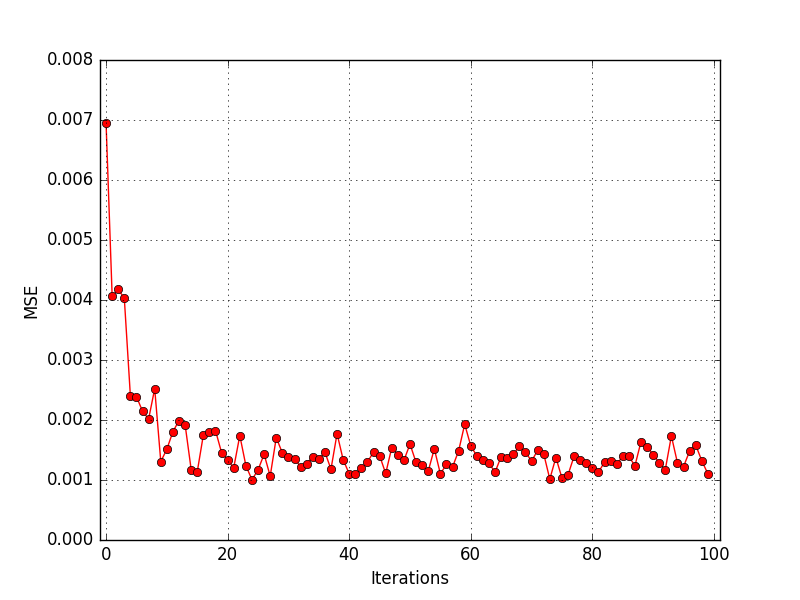
\includegraphics[width=0.8\textwidth]{iterations}
% where an .eps filename suffix will be assumed under latex, 
% and a .pdf suffix will be assumed for pdflatex; or what has been declared
% via \DeclareGraphicsExtensions.

\caption{Iterations versus validation loss.}
\label{fig:trainingMSE}

\end{figure}

\begin{figure}[!htpb]
\centering
\subfloat{
\includegraphics[scale=0.5]{samples/0}} 
\hspace*{0.4in} % separation between the subfigures
\subfloat{
\includegraphics[scale=0.5]{samples/00}}
\\
\subfloat{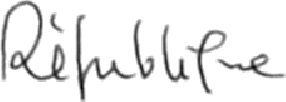
\includegraphics[scale=0.5]{samples/4}} 
\hspace*{0.4in} % separation between the subfigures
\subfloat{
\includegraphics[scale=0.5]{samples/04}}
\\
\subfloat{
\includegraphics[scale=0.5]{samples/10}} 
\hspace*{0.4in} % separation between the subfigures
\subfloat{
\includegraphics[scale=0.5]{samples/010}}
\\
\subfloat{
\includegraphics[scale=0.5]{samples/23}} 
\hspace*{0.4in} % separation between the subfigures
\subfloat{
\includegraphics[scale=0.5]{samples/023}}
\\
\addtocounter{subfigure}{-8}
\subfloat[Synthetic Handwritten Manuscript]{
\includegraphics[scale=0.5]{samples/30}}
\hspace*{0.4in} % separation between the subfigures
\subfloat[Expected Real Manuscript - Groundtruth]{
\includegraphics[scale=0.5]{samples/030}} 


\caption{A not cherry-picked selection of synthetic manuscripts produced using our proposed method alongside the expected output, i.e. the groundtruth.} \label{fig:resultingsamples}
\end{figure}

In order to make an objective evaluation of the quality of the synthetic generation, in the context of handwritten signatures, we performed a machine-oriented evaluation. In the next chapter, we describe the protocol we followed and then we report an objective measure of the quality of our proposed method based on this experimental setup.

%!TEX root = ../dissertation_vkslm.tex

\chapter{Experimental Evaluation}\label{ch:exp}

In order to evaluate the quality of the synthetic signatures generated by our system we follow the same protocol presented on the work of Diaz \cite{diaz2014generation}. Namely we use a state-of-the-art offline verification system and a dataset comprising both online and offline signatures in order to train the verification system to evaluate the synthetic signatures.

The goal of the experiments is to measure the quality of the synthetic signatures taking into account an offline verification system performance. The questions raised are \begin{inlinelist}
  \item is the synthetic signatures system performance similar to the real offline signatures performance?
  \item is the performance even if the enrollment protocol changes?
  \item is it feasible to increase the number of samples at the enrollment stage with synthetic signatures? 
\end{inlinelist}



\section{Off-line signature verification system}
The system used for the evaluation of the real and synthetic signatures is a Linear SVM classifier and is based on a state of the art feature extraction approach  \cite{hafemann2017learning}. The feature extraction system \footnote{https://www.etsmtl.ca/Unites-de-recherche/LIVIA/Recherche-et-innovation/Projets/Signature-Verification} uses ideas from transfer learning and multi-task learning to learn features using Convolutional Neural Networks (CNN).

\subsection {Support Vector Machine} 
SVMs represent a special class of linear classifiers. In order to classify a pattern as
belonging to one of two classes, an SVM constructs a plane such that it maximally separates the margin between the two classes, as it can be seen in Figure \ref{fig:svm}. For this reason, SVMs are also referred to as maximum margin classifiers.

\begin{figure*}[!htb]
\centering
 \subfloat[the data can be separated using different lines]{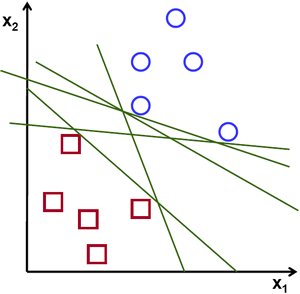
\includegraphics[width=2.3in]{separating-lines}} 
\hspace*{0.5in} % separation between the subfigures
\subfloat[the SVM strives for the optimal line, which maximally separates the margin between the two classes of data] {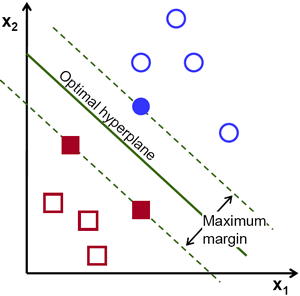
\includegraphics[width=2.3in]{optimal-hyperplane}}

\caption{Illustration of several separating lines and an optimal line.} \label{fig:svm}
\end{figure*}

\subsection {Feature Learning} 
As discussed in Chapter \ref{ch:nndl}, one of the advantages of using deep learning techniques is
not requiring to design feature extractors, but instead let the model learn them. The offline signature verification system feature extractor takes advantage of this concept. 


\section{Evaluation Database}


The evaluation experiments were carried out on the BiosecurID
database \cite{biosecurid}. This multimodal database was made publicly available containing signatures of 132 subjects. Signatures were
captured using a special digital inking pen on a paper placed
over a digitizing tablet. Consequently, both versions, online and
offline, of the exact same real signature were acquired at
the same time. This characteristic, therefore, makes BiosecurID the ideal benchmark for the experimental evaluation conducted in this work.

The signatures were captured in 4 sessions
distributed over 4 months. Each subject signed 4 times and
forged 3 signatures per session, thus leading to each subject having 4 genuine signatures x 4 sessions = 16 genuine samples and 3 signature forgeries x 4 sessions = 12 skilled forgeries. 

MCYT This dataset includes 75 signers collected at four different Spanish
universities. The corpus includes 15 genuine and 15 deliberately forged signatures
acquired in two sessions. All the signatures were acquired with the same inking pen
and the same paper templates. The paper templates were scanned at 600 dpi with 256
grey levels.


\section{Experimental Protocol}
In order to answer the questions stated at the beginning of this section and accomplish a fair comparison of our work and the state of the art, we follow the same experiment protocol proposed by Diaz \cite{diaz2014generation}. Two different experiments are carried out. The Experiment 1 focus on evaluating the synthetic signatures performance in comparison to real signatures and the Experiment 2 evaluates the feasibility of synthetically increasing the number of samples available in a dataset. 

For both experiments the BiosecurID dataset is split into two subsets. The first 90 users are separated as the enrollment set, used to compute the genuine and skilled impostor scores. The remaining 42 authors are considered as the test set and are used to compute the random impostor scores. The performance is evaluated in terms of equal error rate (EER), which is the point in the Detection Error Tradeoff curve (DET) where the false acceptance rate equals the false rejection rate.

\subsection{Experiment 1}

Two different protocols have been considered to
compute the 90 user enrolled models:
\begin{inlinelist}
  \item a mono-session approach, uses the four samples of the first acquisition session
  \item a multi-session approach, uses one sample of each of the 4 acquisition sessions
\end{inlinelist}.

In both cases, genuine scores are computed matching the non-enrolled genuine samples of the subject (12) to the enrolled model (90×12 = 1080 genuine scores). Random impostor scores are calculated comparing the first sample of the test subjects to the
enrolled model, leading to 90×42 = 3780 random impostor scores, and skilled impostor scores are calculated with the skilled forgeries samples of the enrolled users
(12 per subject) to the enrolled model (90×12 = 1080 skilled impostor scores).

\begin{figure}[!htb]
\centering
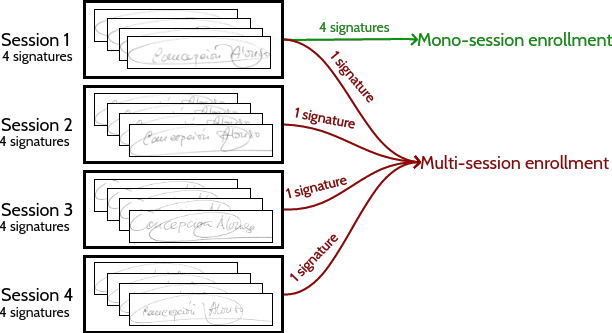
\includegraphics[width=\textwidth]{multi-and-mono}
% where an .eps filename suffix will be assumed under latex, 
% and a .pdf suffix will be assumed for pdflatex; or what has been declared
% via \DeclareGraphicsExtensions.
\caption{The proposed approach diagram and an example of the synthetic signature generation.}
\label{fig:multiandmono}
\end{figure}

\subsection{Experiment 2}

This experiment is designed to assess whether synthetically increasing the enrollment dataset leads to a better recognition performance. Three different enrollment sets are considered in this experiment: 
\begin{itemize}
  \item 4 real samples belonging to the
  first acquisition session
  \item 8 real samples belonging to the first and
  the second sessions
  \item 4 real samples belonging
  to the first session plus 4 synthetic samples belonging
  to the second session.
\end{itemize}

\section{Performance Assessment}

AHSVS efficiency is quantitatively measured by two rates: False Rejection Rate (FRR) which is the percentage of genuine signatures treated as forgeries, and False
Acceptance Rate (FAR) which is the percentage of forged signatures treated as
genuine. 

A derived metric usually reported is the Average Error rate (AER) which is the average of FAR and FRR. Moreover, when experimenting an AHSVS, the trade-off between FRR and FAR must be taken into account based on the type of application and other aspects related to where the system is used. When the decision threshold of a system is set to have the FRR approximately equal to the FAR, the Equal Error Rate (EER) is calculated.

%Besides quantitative results, the performance can be also compared and visualized using graphs. Receiver operating characteristics (ROC) graphs have been used increasingly in machine learning and data mining research \cite{fawcett2006introduction}. Inicialmente, a curva ROC foi desenvolvida para demonstrar as relações sinal-ruído,
%interpretando o sinal como verdadeiros positivos (sensibilidade) e o ruído, os falsos positivos
%(especificidade). Assim, a leitura da curva ROC é de um gráfico de sensibilidade ou taxas de
%verdadeiros positivos versus taxa de falsos positivos, como apresentado na Figura 26. Os
%gráficos ROC são bidimensionais, estando o eixo Y com os valores verdadeiros positivos e o
%eixo X preenchido com os valores da taxa falsos positivo.
%
%O objetivo da ferramenta curva ROC é atingir a representação perfeita do experimento,
%considerando o conjunto de amostras analisado.
%O objeto de estudo tem sua avaliaçãoidentificada pela localidade do ponto no gráfico. Quão mais próximo o ponto estiver do eixo Y,
%melhor será o resultado. Assim, a diagonal traçada do ponto (0,0) ao ponto (1,1) serve de
%direcionamento para identificar quais são os melhores resultados, estes localizados
%predominantemente acima da reta [FAWCELT, 2006]. 
%
%A métrica utilizada no estudo do ICDAR 2009 [BLANKERS et al, 2009] foi a Detection
%Error Trade-off curve (DET) [MARTIN, 1997] (gráfico visualizado na Figura 28). Esta métrica
%é mais conhecida como a curva DET. Esta curva corresponde a um gráfico que estabelece uma
%relação entre as taxas de erro diferentemente da curva ROC. A curva é definida como a linha
%contendo os pontos onde x = y, ou seja, posição onde os erros FRR e FAR possuem o mesmo
%valor. Assim, o gráfico é gerado baseando-se na taxa EER. No gráfico DET o melhor resultado
%está localizado o mais próximo do eixo inicial (o ponto 0 (zero)). O mais próximo apresenta,
%assim, o menor erro de classificação. Esta métrica foi utilizada pelo ICDAR para definir o
%algoritmo de classificação da competição com o melhor EER nos problemas de verificação de
%assinaturas nos modos off-line e on-line.

%\section{Statistical Evaluation}



%!TEX root = ../dissertation_vkslm.tex

\chapter{Results} \label{ch:results}

As described in Chapter \ref{ch:exp}, two different experiments were
carried out to evaluate the synthetic signatures generated with our proposed method. Namely, we intend to measure how close the synthetic signatures are to real ones and to verify the feasibility of increasing the enrollment dataset with synthetic signatures. The goal of the experiments are:
\begin{itemize}
  \item Measure the quality of the synthetic images;
  \item Assess whether using synthetic signatures effects the recognition performance of an offline signature verification system; and
  \item Analyze the feasibility of using real and synthetic signatures
  on the enrollment set.
\end{itemize}

We compare our results with a state-of-the-art method, particularly the approach proposed by Diaz \textit{et al.} \cite{diaz2014generation}. Specifically, our proposed method is compared with the ``Image enhanced'' synthetic signatures made available as part of the BiosecurID \cite{biosecurid} dataset. The reported EER is achieved for both approaches in the same experimental conditions.

The recognition rates of three types of offline signatures are reported: 
\begin{inlinelist}
  \item real offline signatures, which are the corresponding real offline samples of the online signatures used to generate the synthetic samples, they serve us as a ground-truth, i.e., the ideal synthetic signature should be similar to it;
  \item synthetic signatures generated with the method proposed by Diaz \textit{et al.} \cite{diaz2014generation};
  \item synthetic signatures created with our proposed method
\end{inlinelist}.

\section{Synthetic Signatures in Comparison to Real Signatures - Experiment 1}
In order to evaluate the performance of the synthetic signature signatures described in Chapter \ref{ch:method} and the state-of-the-art, two scenarios were experimented: 
\begin{itemize}
\item Mono-session: signatures from the first session on the enrollment set; and
\item Multi-session: one signature per session.
\end{itemize}


\begin{table}[!htb]
%% increase table row spacing, adjust to taste
\renewcommand{\arraystretch}{1.3}
% if using array.sty, it might be a good idea to tweak the value of
% \extrarowheight as needed to properly center the text within the cells
\caption{EER for real, synthetic samples from Diaz \textit{et al.} \cite{diaz2014generation} and our proposed method synthetic offline signatures, for all the approaches considered under the two possible scenarios (i.e., random and skilled forgeries)}
\label{exp1_results_table}
\centering
%% Some packages, such as MDW tools, offer better commands for making tables
%% than the plain LaTeX2e tabular which is used here.
\begin{tabular}{|l|l|l|l|}
    \hline
    \multicolumn{1}{|c|}{\multirow{2}{*}{\textbf{Mode}}} & \multicolumn{3}{c|}{\textbf{Skilled Forgeries}}          \\ \cline{2-4} 
    \multicolumn{1}{|c|}{}                               & \textbf{Real} & \textbf{Diaz \textit{et al.}} & \textbf{Proposed method} \\ \hline
    \textbf{mono-session}                                & 20.28\%            & 23.19\%            & 18.38\%                       \\ \hline
    \textbf{multi-session}                               & 17.59\%            & 22.27\%            & 16.48\%                       \\ \hline
    \multirow{2}{*}{}                                    & \multicolumn{3}{c|}{\textbf{Random Forgeries}}           \\ \cline{2-4} 
    & \textbf{Real} & \textbf{Diaz \textit{et al.}} & \textbf{Proposed method} \\ \hline
    \textbf{mono-session}                                & 9.07\%            & 10.65\%            & 9.99\%                       \\ \hline
    \textbf{multi-session}                               & 5.60\%            & 10.00\%            & 6.48\%                       \\ \hline
\end{tabular}

\end{table}

Table \ref{exp1_results_table} shows the EER achieved by the
real and the synthetic signatures databases. We observe that under the skilled forgeries scenario our proposed method synthetic signatures EERs yields better performance than both the real dataset and the synthetic signatures generated by Diaz \textit{et al.}. On the random forgeries test, we can identify that, under the random forgeries scenario, the EER results achieved by the real, and both types of synthetic signatures are close to each other. Specifically, under the mono-session scenario, the system's performance for the real signatures was 9.07\%, while the synthetic samples from Diaz \textit{et al.} and our proposed method achieved 10.65\% and 9.99\%, respectively. However, on the multi-session test, the signatures from Diaz \textit{et al.} achieved 10.00\% ERR, while the real signatures and our proposed method EER was 5.60\% and 6.48\%, respectively.


In Figure \ref{exp1} (left - mono-session, right - multi-session) we
may observe that the behavior of the system with real (gray dotted) and our proposed method synthetic signatures are quite similar, regardless of
the training protocol or the scenario considered. Nevertheless, our proposed method synthetic samples achieved a better discriminative power for skilled forgeries.
\begin{figure*}[!htb]
    \centering
    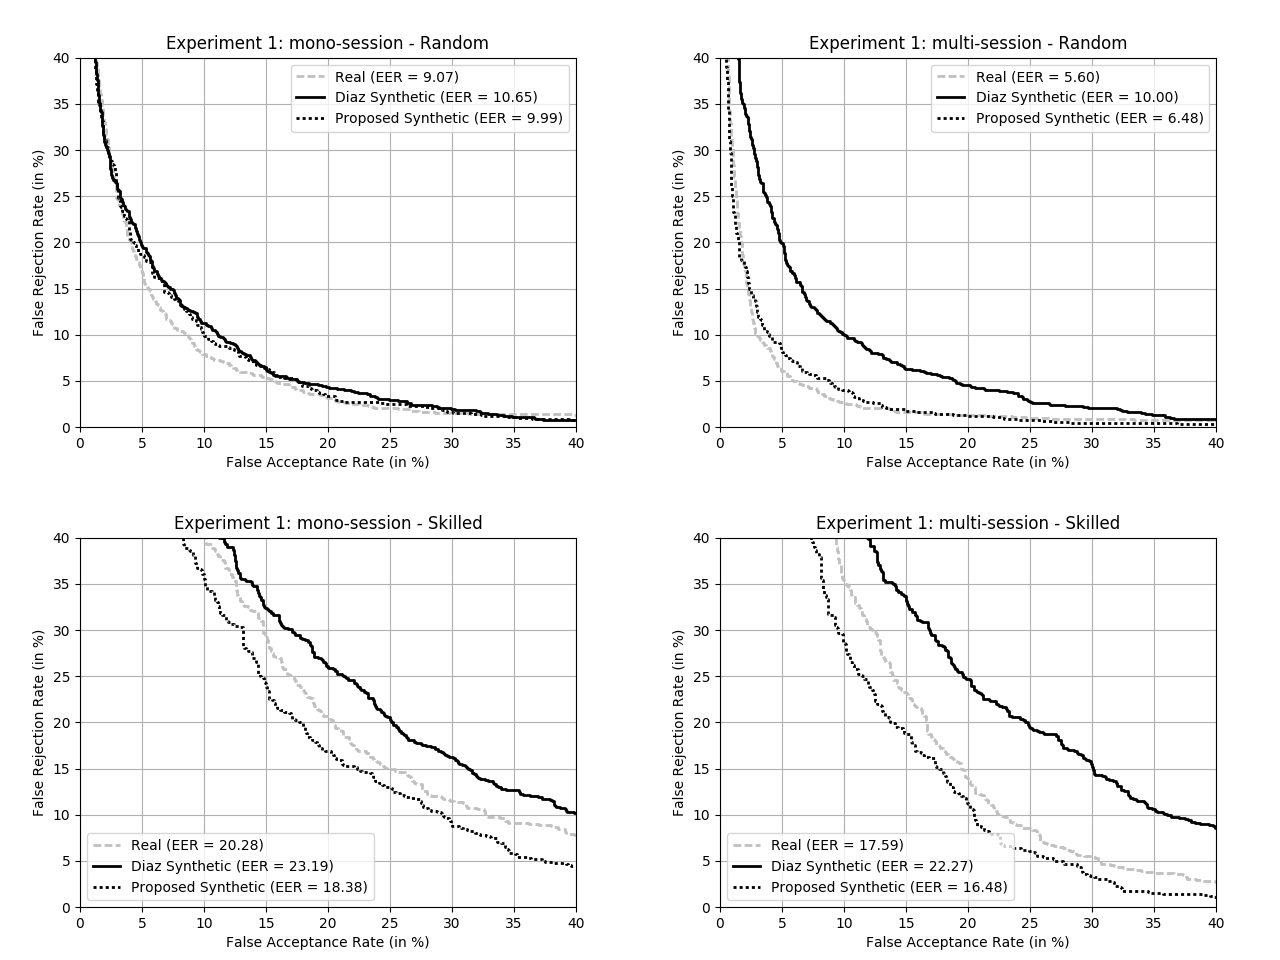
\includegraphics[width=1.05\textwidth]{rocs/experiment1}
    % where an .eps filename suffix will be assumed under latex, 
    % and a .pdf suffix will be assumed for pdflatex; or what has been declared
    % via \DeclareGraphicsExtensions.
    \caption{DET curves for real offline signatures and synthetic signatures (from Diaz \textit{et al.} and our proposed method), for the first experiment (mono-session and multi-session enrollment), for the two scenarios considered (random and skilled impostors)}
    \label{exp1}
\end{figure*}

Moreover, in Figure \ref{fig:box_exp1} we can see that when running the experiments 30 times, the results are consistent, with a low dispersion around the average. We can notice that our proposed method is able to produce synthetic signatures comparable to the real signatures.


\begin{figure*}[!htb]
\centering
 \subfloat[mono-session - random forgeries]{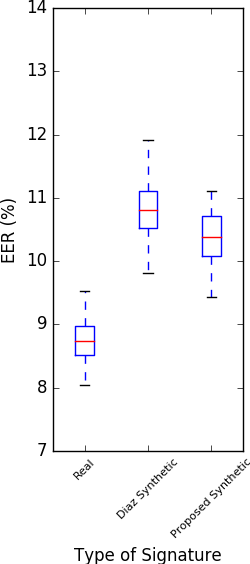
\includegraphics[width=1.3in]{boxplot/mono-random.png}} 
\hspace*{0.2in} % separation between the subfigures
\subfloat[mono-session - skilled forgeries] {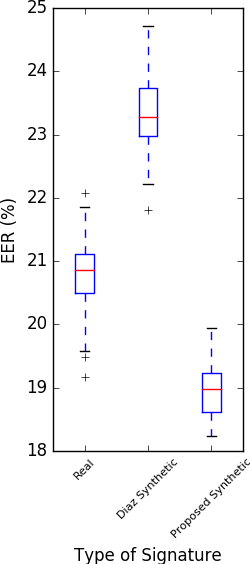
\includegraphics[width=1.3in]{boxplot/mono-skilled.png}}
\hspace*{0.3in} % separation between the subfigures
\subfloat[multi-session - random forgeries]{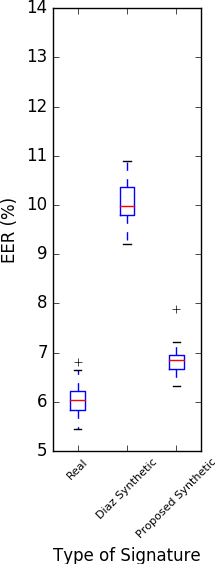
\includegraphics[width=1.3in]{boxplot/multi-random.png}} 
\hspace*{0.2in} % separation between the subfigures
\subfloat[multi-session - skilled forgeries] {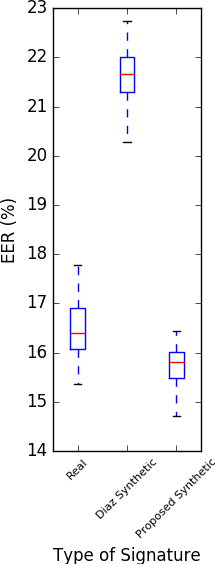
\includegraphics[width=1.3in]{boxplot/multi-skilled.png}}
\caption{Boxplot comparison for running 30 times the Experiment 1 - mono-session scenario and multi-session. (a) mono-session scenario, random forgeries, (b) mono-session scenario, skilled forgeries, (c) multi-session scenario, random forgeries, (d) multi-session scenario, skilled forgeries. } \label{fig:box_exp1}
\end{figure*}

\section{Feasibility of Synthetically Increasing the Enrollment Samples - Experiment 2}
In the last experiment, the feasibility of synthetically
increasing the signature verification enrollment set is analyzed. As it is described in
Chapter \ref{ch:exp}, three different enrollment sets are considered. The DET curves for the mixed enrollment (real + synthetic, gray dashed line) is shown in Figure \ref{fig:exp2} and the summary of the results is presented in Table \ref{exp2_results_table}. We can observe that a better performance compared to the case with only four real
enrolled samples (black line). Specifically, the EER decreases from 10.26\% to 9.74\% on the random forgeries scenario and from 21.55\% to 19.17\% for skilled forgeries, respectively. The addition of synthetic samples for training thus leads to better recognition results.
\begin{figure}[!htb]
    \centering
    

    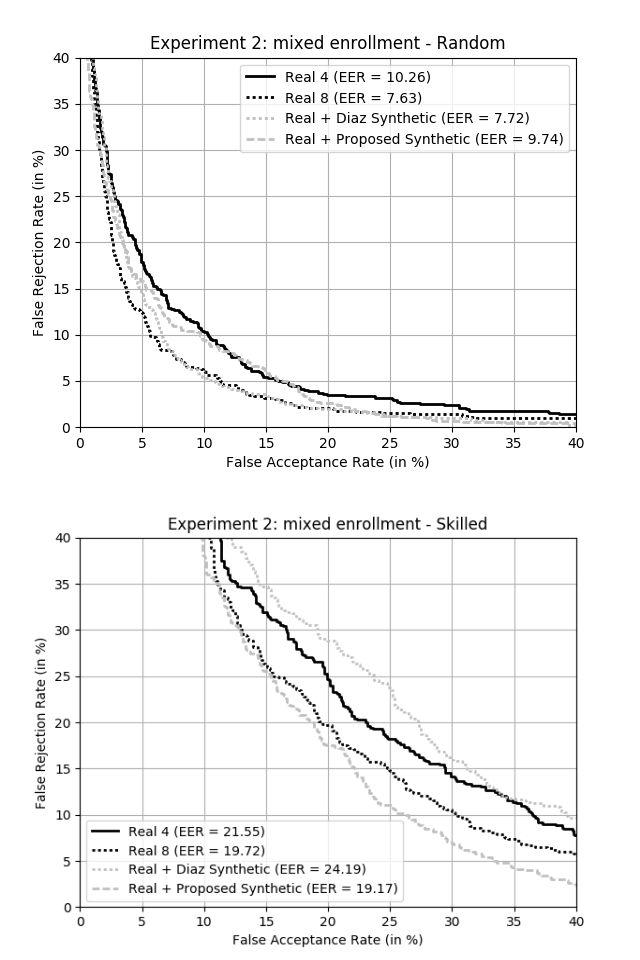
\includegraphics[width=4.5in]{rocs/experiment2}
    % where an .eps filename suffix will be assumed under latex, 
    % and a .pdf suffix will be assumed for pdflatex; or what has been declared
    % via \DeclareGraphicsExtensions.
    \caption{DET curves for real offline signatures and synthetic signatures (from Diaz \textit{et al.} and our proposed method), for the second experiment, for the two scenarios considered (random and skilled impostors)}
    \label{fig:exp2}
\end{figure}

\begin{table}[!htb]
    %% increase table row spacing, adjust to taste
    \renewcommand{\arraystretch}{1.3}
    % if using array.sty, it might be a good idea to tweak the value of
    % \extrarowheight as needed to properly center the text within the cells
    \caption{EER for real, synthetic samples from Diaz \textit{et al.} \cite{diaz2014generation} and our proposed method synthetic offline signatures for the Experiment 2 under the two possible scenarios, i.e., random (RF) and skilled forgeries (SF)}
    \label{exp2_results_table}
    \centering
    %% Some packages, such as MDW tools, offer better commands for making tables
    %% than the plain LaTeX2e tabular which is used here.
    \begin{tabular}{|l|l|l|}
        \hline
        \multicolumn{1}{|c|}{\textbf{Genuine Training}} & \multicolumn{1}{c|}{\textbf{SF}} & \textbf{RF} \\ \hline
        \textbf{4 real samples}                                         & 21.55\%                     & 10.26\%                         \\ \hline
        \textbf{4 real + 4 real samples}                       & 19.72\%                      & 7.63\%                        \\ \hline
        \textbf{4 real + 4 synthetic from Diaz \textit{et al.}}                           & 24.19\%                         & 7.72\%                \\ \hline
        \textbf{4 real + 4 synthetic from the Proposed Method}                           & 19.17\%         & 9.74\%                        \\ \hline
    \end{tabular}

\end{table}

It should also be noted that the behavior of the mixed enrollment is similar to the scenario with eight real enrolled samples (i.e., using eight real samples instead of
four real and four synthetic, black line) for skilled forgeries, and even yields a small improvement on the skilled forgery recognition rates. 

Furthermore, we can see in Figure \ref{fig:boxexp2} that when running the experiments for 30 times, the results of our proposed method has a consistent mean, with
a lower variance around the average. In addition to achieving a comparable EER to using 8 real samples on the enrollment set on the random forgery and skilled forgery scenario.

\begin{figure}[!htb]
\centering
 \subfloat[mixed enrollment - random forgeries]{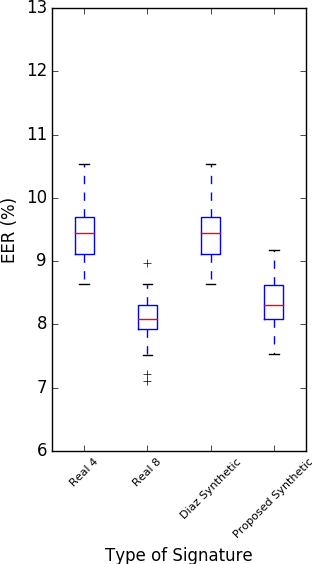
\includegraphics[width=2.0in]{boxplot/mixed-random.png}} 
\hspace*{0.8in} % separation between the subfigures
\subfloat[mixed enrollment - skilled forgeries] {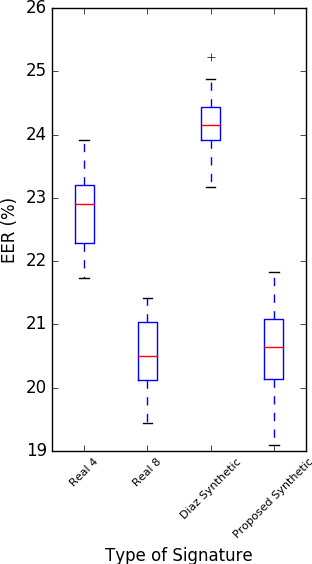
\includegraphics[width=2.0in]{boxplot/mixed-skilled.png}}
\caption{Boxplot comparison for Experiment 2: mixed enrollment - (a) random forgeries and (b) skilled forgeries. } \label{fig:boxexp2}
\end{figure}

It is possible for us to conclude that it is feasible to use our proposed system to generate synthetic signatures from dynamic data, when complementary online samples are available, to increase an offline signature dataset, aiming to improve the recognition rate of offline verification systems.





%!TEX root = ../dissertation_vkslm.tex

\chapter{Conclusion and Future Works}\label{ch:conclusion}
This work proposes a method to synthesize offline signatures from dynamic information as a supervised learning task. We propose a Fully Convolutional Neural Network to learn an end-to-end mapping of online manuscripts to the static domain, taking advantage of the data present in the IRONOFF dataset during the training phase of the Neural Network. 

We show that, in contrast to what has already been proposed, it is possible to model the "online to offline signature" as a learning from data task. Our Deep Neural Network model learns how the online biometric data must be used to build the grayscale signature image. Furthermore, we also observe that our proposed method synthetic offline signatures offer a verification performance similar to the one offered by real signatures and we show that the synthetic signatures present high discriminative power when used to increase the enrollment set under the skilled forgeries scenario. 

Future work can explore the optimization of the hyper-parameters of the FCN (such as the number of layers, number of neurons per layer) since these hyper-parameters were fixed during the experiments in the present work. Besides, we intend to explore the combination of real online and synthetically generated offline signatures using the proposed method, when only the online information is available, towards improved recognition results on a dynamic signature verifier.

Another improvement to the current work is the integration of other dynamic features in addition to the pressure on the input of the network, such as the velocity. Moreover, one could also design a model to synthesize offline signatures with bigger resolution.
% ----------------------------------------------------------
% ELEMENTOS PÓS-TEXTUAIS
% ----------------------------------------------------------
\postextual
% ----------------------------------------------------------

% ----------------------------------------------------------
% Referências bibliográficas
% ----------------------------------------------------------
\bibliography{library}
% ----------------------------------------------------------
% Glossário
% ----------------------------------------------------------
%
% Consulte o manual da classe abntex2 para orientações sobre o glossário.
%
%\glossary

% ---
% Apêndices e Anexos
% ---
 \begin{apendicesenv}

%\chapter{Preprocessed IRONOFF samples}
%a
%\chapter{Neural Network model weights}
%a
%\chapter{Synthetic Samples from BiosecureID online signatures}
%a
%\chapter{Extracted Features}
%a
% ----------------------------------------------------------
\chapter{Publications}

As results of this work, a chapter has been published in the book Handwriting: Recognition, Development and Analysis and a paper has been submitted to the peer-reviewed journal Pattern Recognition Letters.

\textbf{Title:} Datasets for Handwritten Signature Verification: A Survey and a New Dataset, the RPPDI SigData.

\textbf{Authors:} Melo, V.K.S.L., Bezerra, B.L.D., do Nascimento, R.H.S.N., de Moura, G.C.D., Martins, G.L.L.d.S., Pirlo, G., Impedovo, D.

\textbf{In:} Handwriting: Recognition, Development and Analysis, ISBN 978-1-53611-957-2, Nova Science Publishers, New York, 2017

\textbf{Abstract:} As a result of a wide research in automatic handwritten signature verification, multiple data sets and competitions emerged to cover different tasks for online/offline signature verification and signature segmentation from scanned documents. The purpose of this work is to analyze and discuss the most used data sets in the literature in order to find what are the challenges pursued by the community in the past few years. The data sets, which were collected from recent publications and competitions, are described regarding its main characteristics such as the number of authors, signatures per author and the method used for the acquisition phase. We analyzed several databases used for different topics related to either online or offline signature verification. Since we did not find in this review a data set that can be used to explore signature verification considering different acquisition sources and writing conditions, specifically a data set consisting of dynamic signatures taken from multiple devices and static signatures with diverse signing area constraints and background textures, we introduce a new data set acquired from pen tablets, smartphones and scanned from different types of documents. Therefore, researchers can use this new data set not only to investigate the multi-domain signature verification problem but to take into account in their solutions the signature segmentation problem in real world documents with complex backgrounds.

\hspace{0.6in}

\textbf{Title:} A Deep Learning Approach to Generate Off-line Handwritten Signatures Based on On-line Samples

\textbf{Authors:} Melo, V.K.S.L., Bezerra, B.L.D., Impedovo, D., Pirlo, G.

\textbf{(In revision):} Pattern Recognition Letters

\textbf{Abstract:} One of the main challenges of offline signature verification is the absence of large databases. A possible alternative to overcome this problem is the generation of synthetic signature databases. In this work, a novel method for the generation of synthetic off-line signatures based on dynamic information is presented. In contrast to the state-of-the-art, we propose a synthesis approach under the perspective of supervised training, in which our learning model is trained to perform the task of “online signature to offline signature conversion”. The proposed approach is based on a Deep Convolutional Neural Network trained to learn how online handwritten manuscripts of the IRONOFF dataset are transformed into the offline domain. The main goal of the proposed method is to synthetically enlarge existing offline signature datasets based on online signature samples towards an improvement on the recognition rates of offline signature verification systems. For these purposes, a machine-oriented evaluation on the BiosecurID signature dataset is carried out. Through the synthetic samples generated with the proposed method, we show a verification performance similar to the one offered by real authentic signatures and assuring improvements of the Equal Error Rate results in comparison with the current state-of-the-art method.


\end{apendicesenv}

%\begin{anexosenv}


% ---
\chapter{Morbi ultrices rutrum lorem.}
% ---
\lipsum[30]

% ---
\chapter{Cras non urna sed feugiat cum sociis natoque penatibus et magnis dis
parturient montes nascetur ridiculus mus}
% ---

\lipsum[31]

% ---
\chapter{Fusce facilisis lacinia dui}
% ---

\lipsum[32]

\end{anexosenv}



%---------------------------------------------------------------------
% INDICE REMISSIVO
%---------------------------------------------------------------------
\phantompart
\printindex
%---------------------------------------------------------------------

\end{document}
